\label{SAPConfig}
\section{Creation of the Microsoft Azure \acrshort{vm}}
The required Microsoft Azure \acrshort{vm} will be created as described in Appendix \ref{Containers_Azure}. 
The required Azure \acrshort{vm} is shown in Figure \ref{fig:SAPInfra}.

\section{Installation of the SAP environment}
The following components will be installed:

\begin{itemize}
    \item SAP NetWeaver 7.5
    \item Adobe Document Services
    \item Advanced Adapter Engine Extended
    \item Application Server Java
    \item BPM and Event Management
    \item Composition Platform
    \item EP Core
    \item Enterprise Services Repository
    \item PDF Export 
\end{itemize}

\subsection{Preconditions}
\subsubsection{Server information}
\begin{description}
    \item[Local IP] 10.0.1.4
    \item[Public IP] 40.68.22.199
    \item[User] jensdufour
    \item[Password] Bachelorproef2019
    \item[Ports] RDP
    \item[Windows Release] Windows Server 2016 Datacenter Edition
\end{description}   

\subsubsection{Disk layout}
\begin{description}
    \item[SAP EXE (E:)] 128 GB
    \item[DB DISK (F:)] 256 GB
    \item[TEMP SOFT (T:)] 256 GB
\end{description}

\subsubsection{Windows preparations}
\begin{figure}[!htb]
    \begin{subfigure}{0.5\textwidth}
        \captionsetup{width=0.8\linewidth}
        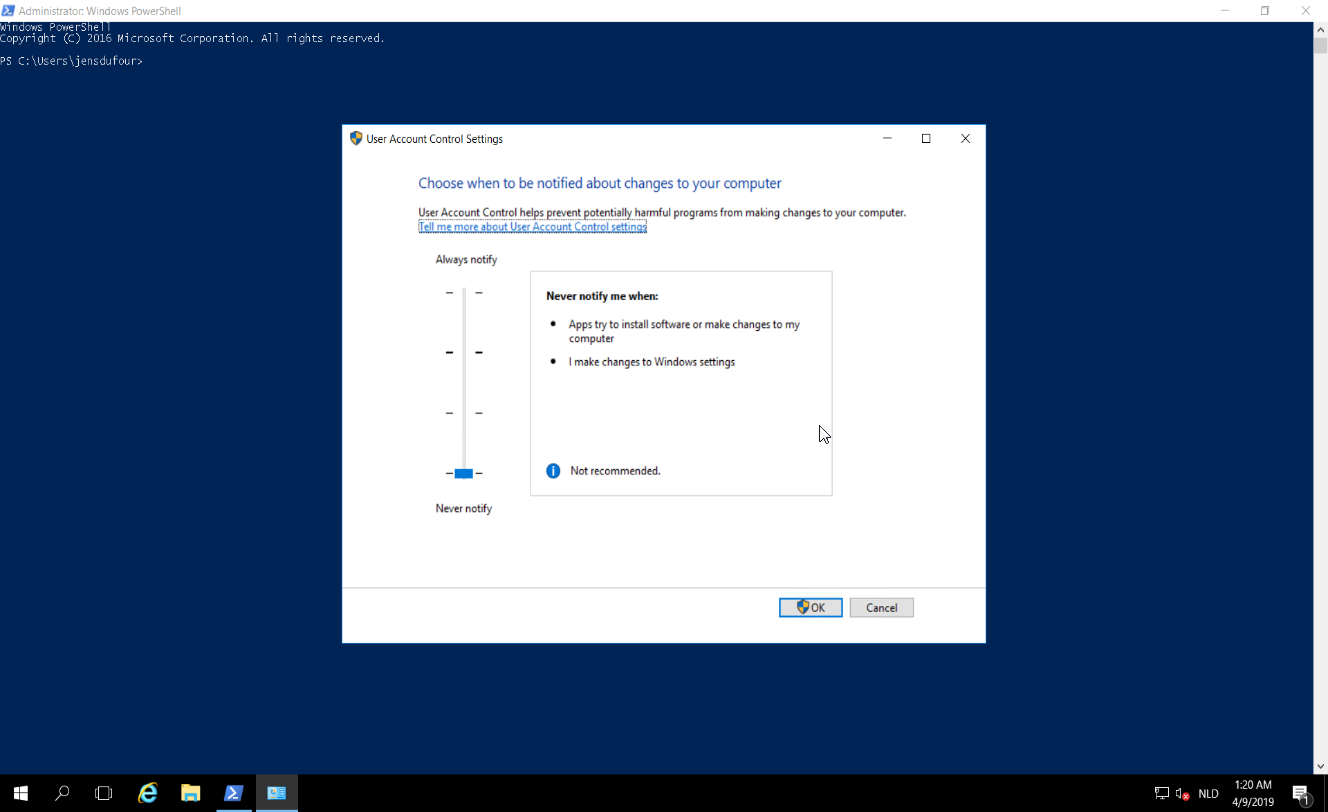
\includegraphics[width=0.9\linewidth]{img/Methodologie/Precondition0.png}
        \centering
        \caption{Disable UAC}
    \end{subfigure}
    \begin{subfigure}{0.5\textwidth}
        \captionsetup{width=0.8\linewidth}
        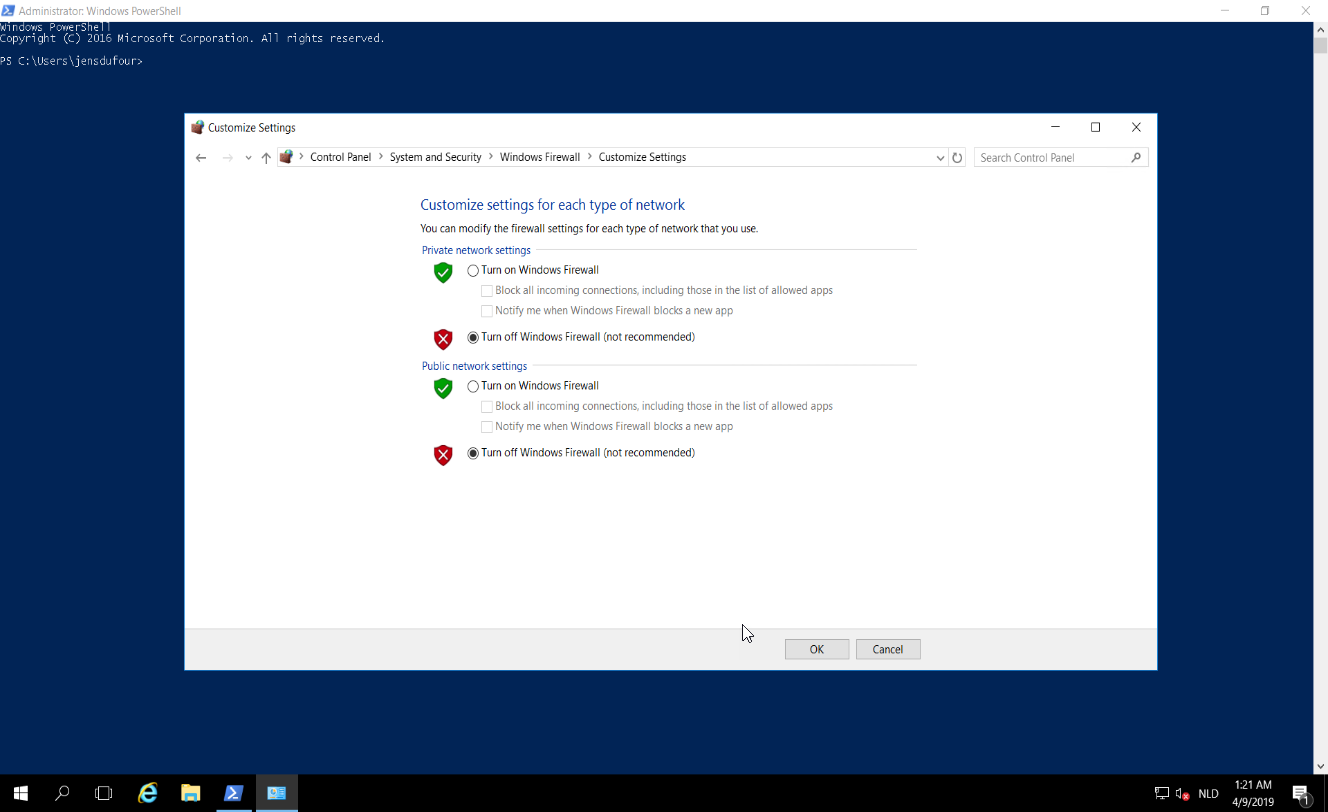
\includegraphics[width=0.9\linewidth]{img/Methodologie/Precondition1.png} 
        \centering
        \caption{Disable Firewall}
    \end{subfigure}
\end{figure}
\begin{figure}[!htb]\ContinuedFloat
    \begin{subfigure}{0.5\textwidth}
        \captionsetup{width=0.8\linewidth}
        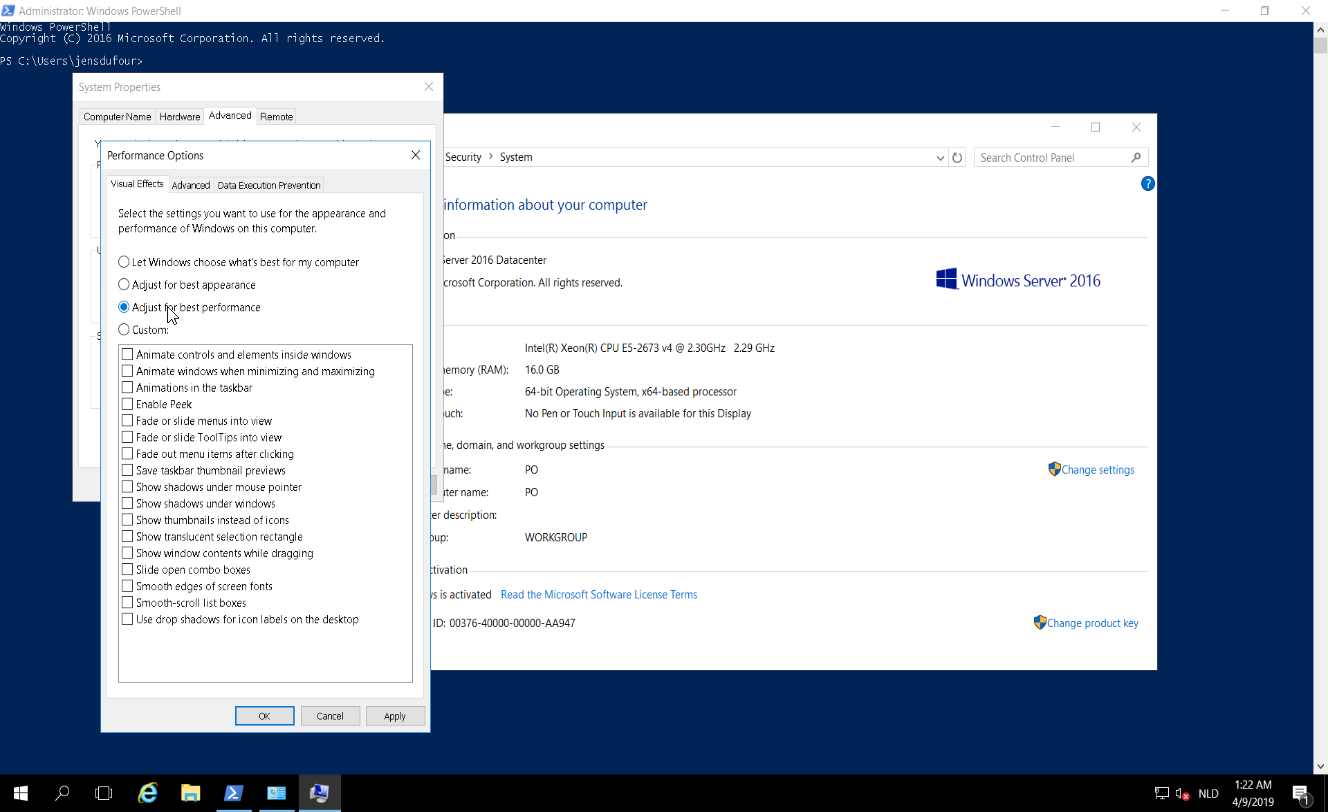
\includegraphics[width=0.9\linewidth]{img/Methodologie/Precondition2.png}
        \centering
        \caption{Adjust visual effects for best performance}
    \end{subfigure}
    \begin{subfigure}{0.5\textwidth}
        \captionsetup{width=0.8\linewidth}
        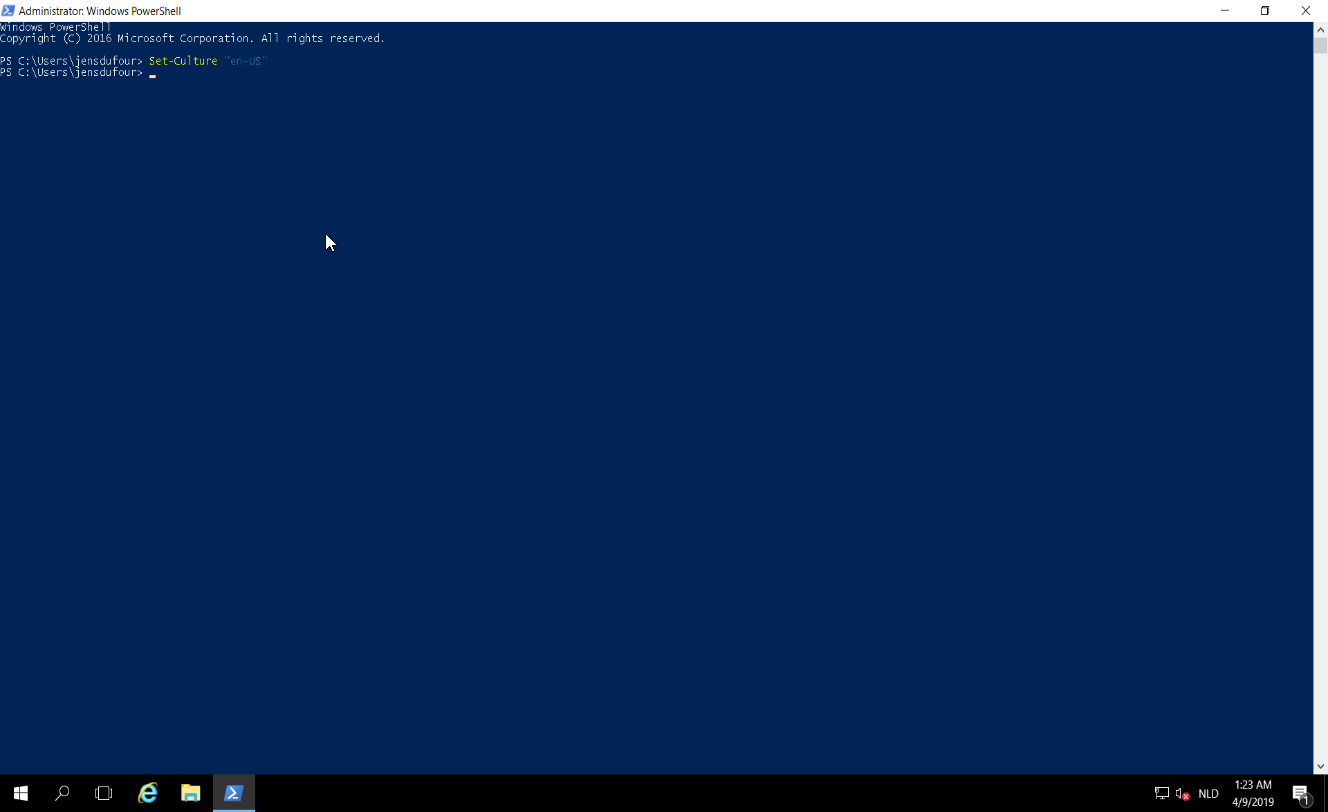
\includegraphics[width=0.9\linewidth]{img/Methodologie/Precondition3.png} 
        \centering
        \caption{Change system locale to EN}
    \end{subfigure}
\end{figure}
\begin{figure}[!htb]\ContinuedFloat
    \begin{subfigure}{0.5\textwidth}
        \captionsetup{width=0.8\linewidth}
        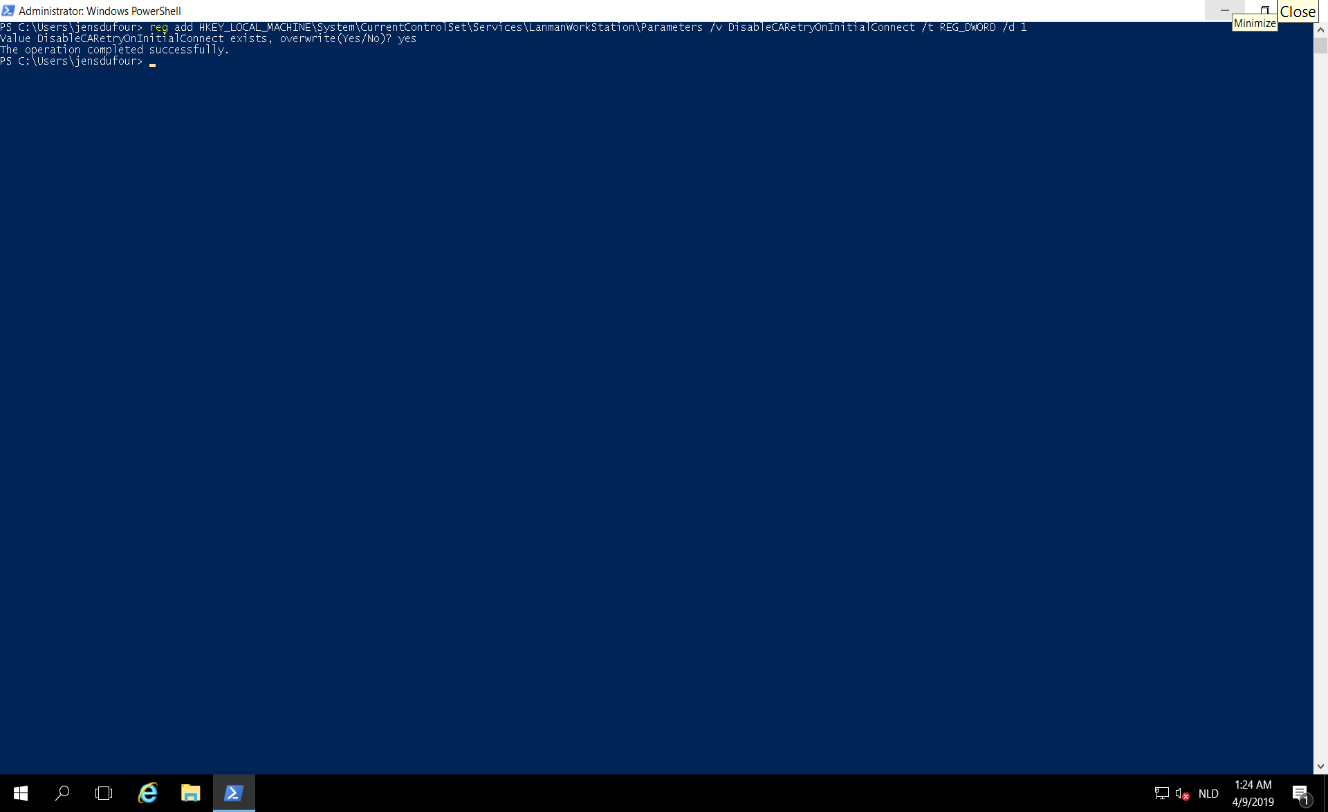
\includegraphics[width=0.9\linewidth]{img/Methodologie/Precondition4.png}
        \centering
        \caption{Accessing time shares / file system}
    \end{subfigure}
    \begin{subfigure}{0.5\textwidth}
        \captionsetup{width=0.8\linewidth}
        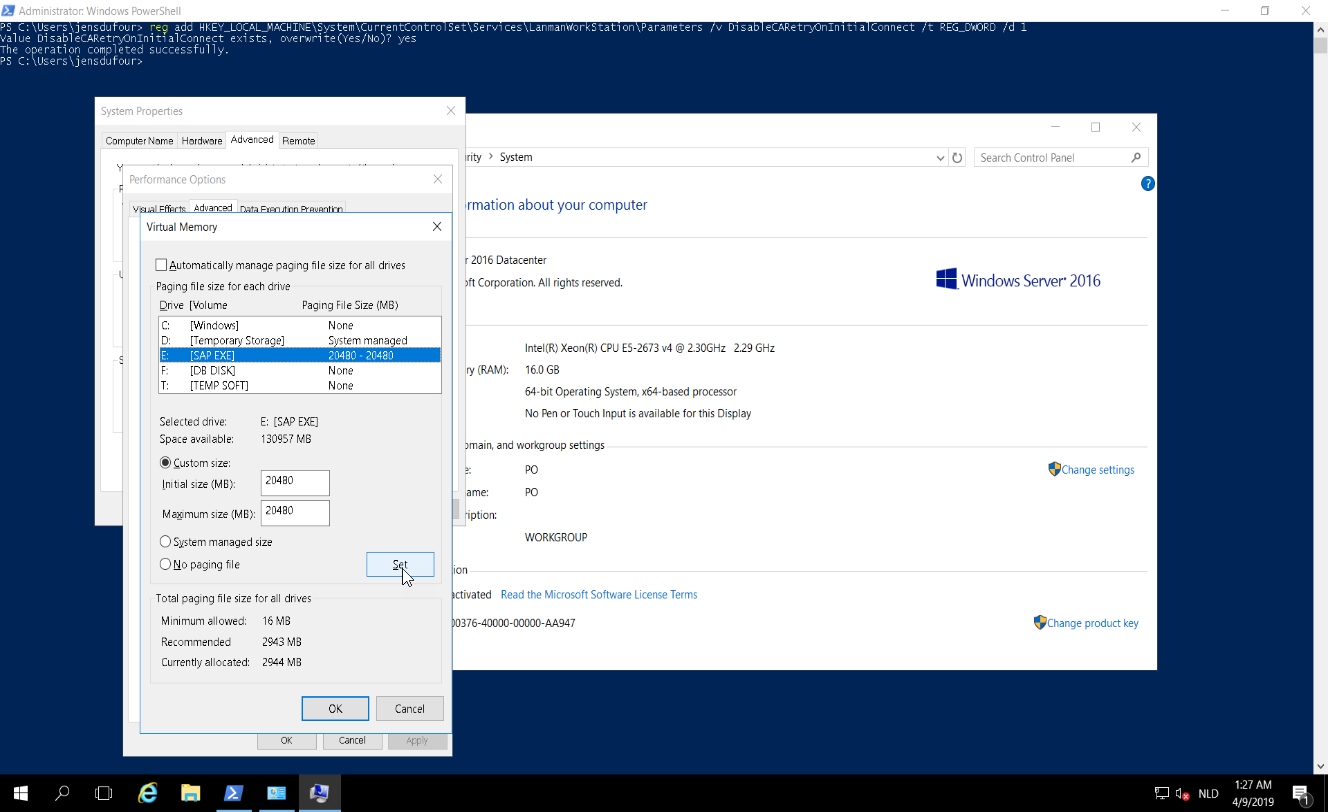
\includegraphics[width=0.9\linewidth]{img/Methodologie/Precondition5.png} 
        \centering
        \caption{Set paging file to 20480}
    \end{subfigure}
\end{figure}
\begin{figure}[!htb]\ContinuedFloat
    \begin{subfigure}{\textwidth}
        \captionsetup{width=0.8\linewidth}
        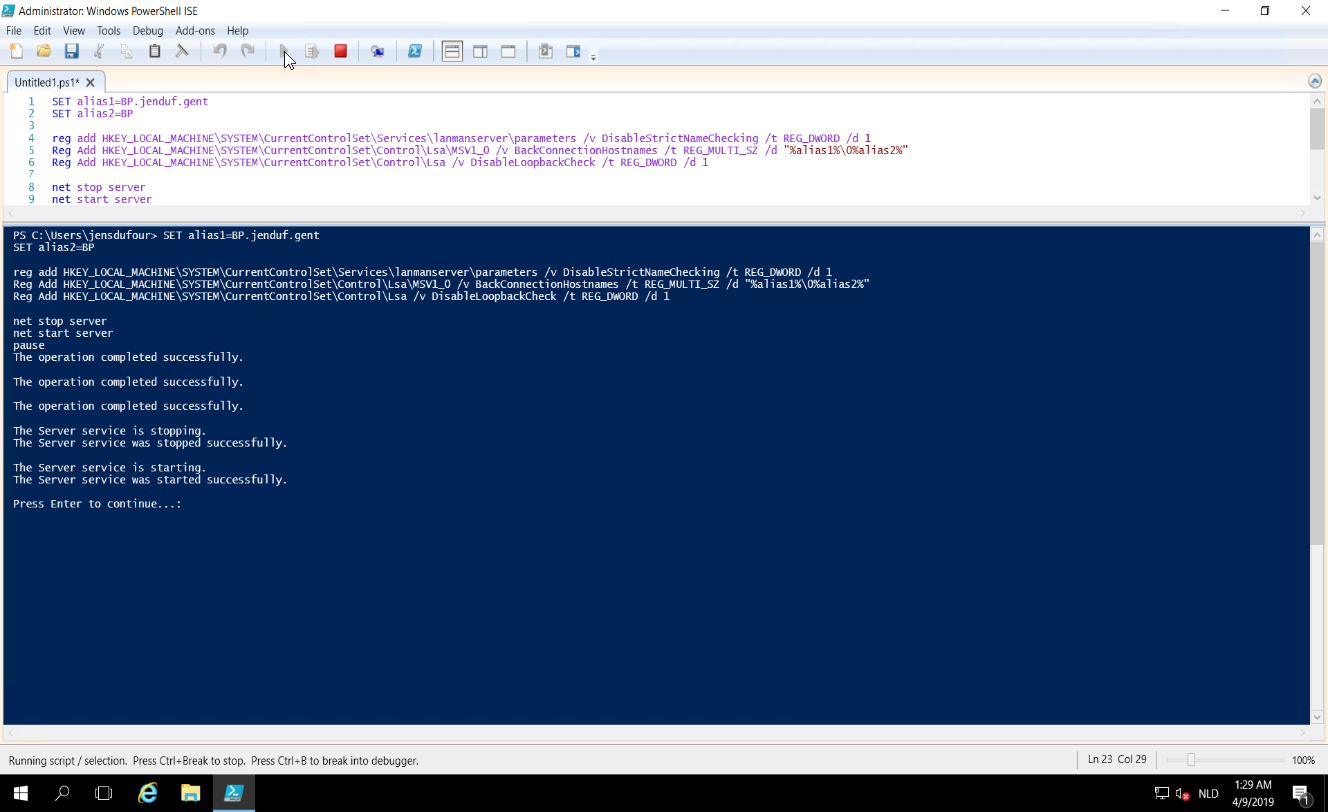
\includegraphics[width=0.9\linewidth]{img/Methodologie/Precondition6.png}
        \centering
        \caption{Setting Virtual Host Names on Windows}
    \end{subfigure}
    \caption[Preconditions SAP]{Preconditions for the installation of the SAP stack}
    \label{fig:Preconditions}
\end{figure}
\clearpage

\subsection{Installation}
\begin{figure}[!htb]
    \begin{subfigure}{0.5\textwidth}
        \captionsetup{width=0.8\linewidth}
        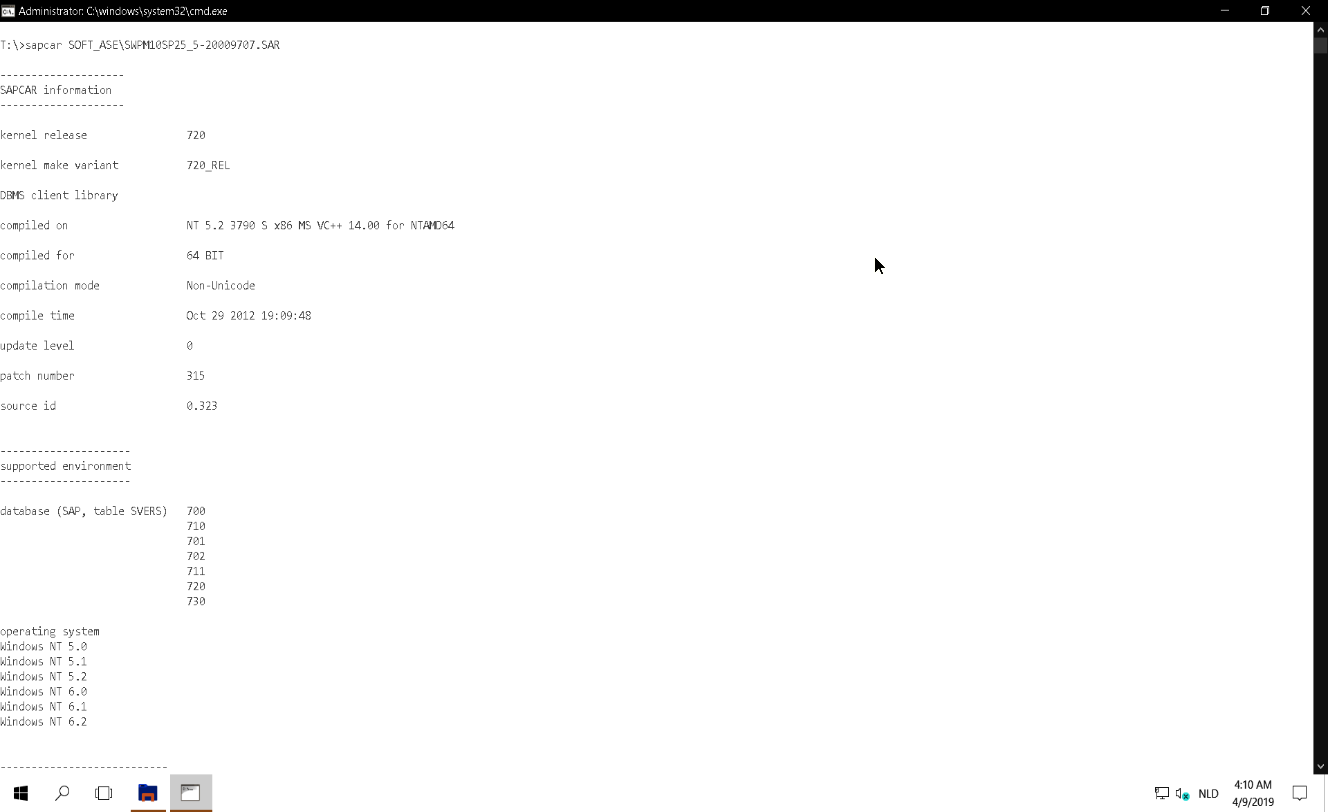
\includegraphics[width=0.9\linewidth]{img/Methodologie/SAP38.png}
        \centering
        \caption{Extract the Software Provisioning Manager using 'SAPCAR'}
    \end{subfigure}
    \begin{subfigure}{0.5\textwidth}
        \captionsetup{width=0.8\linewidth}
        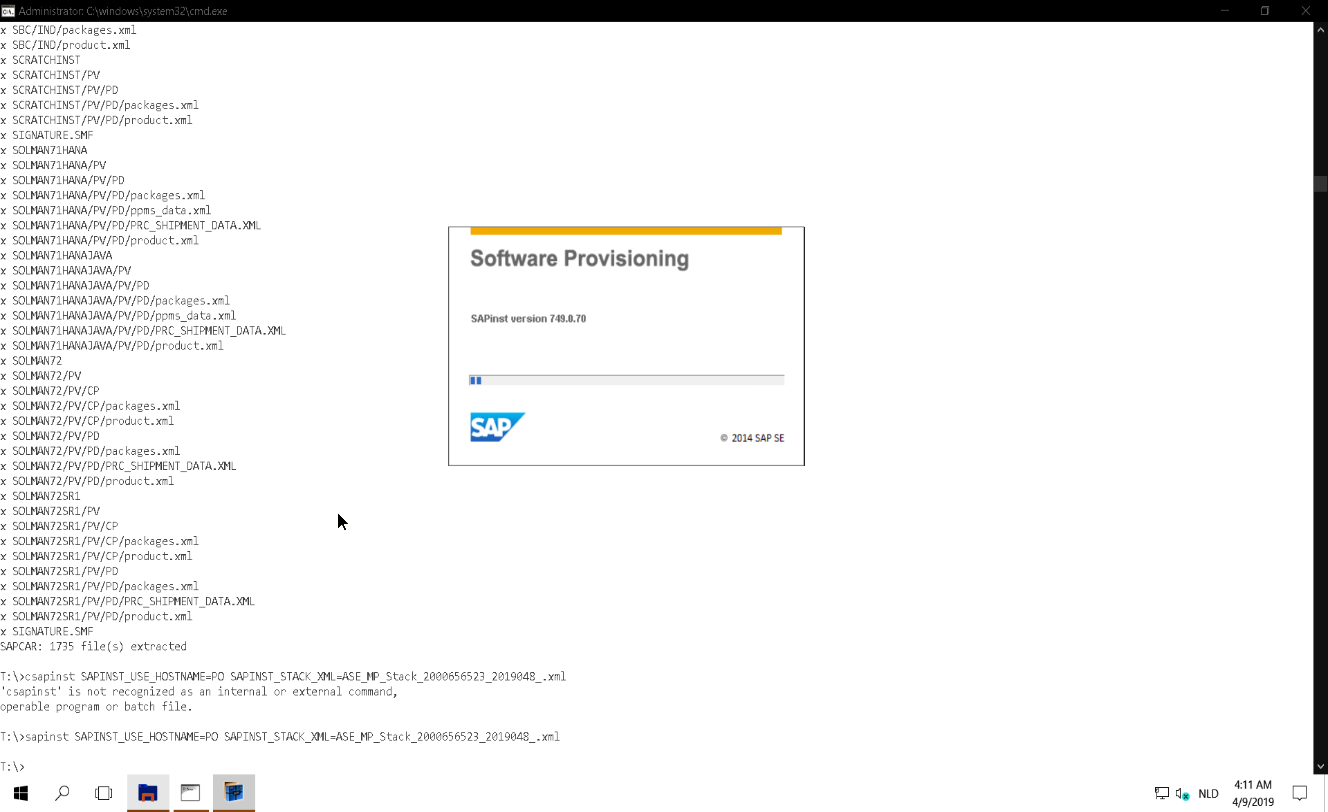
\includegraphics[width=0.9\linewidth]{img/Methodologie/SAP37.png} 
        \centering
        \caption{Start the Software Provisioning Manager}
    \end{subfigure}
\end{figure}
\begin{figure}[!htb]\ContinuedFloat
    \begin{subfigure}{0.5\textwidth}
        \captionsetup{width=0.8\linewidth}
        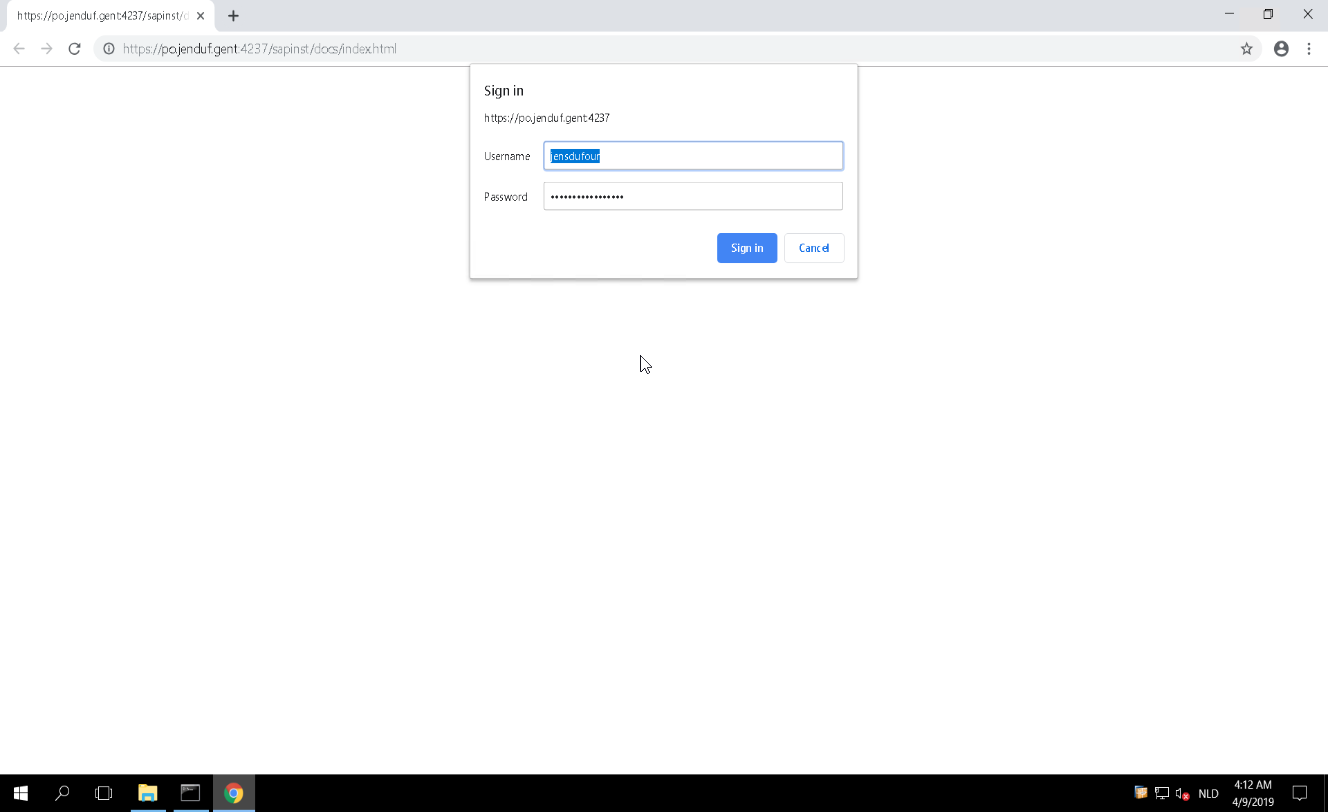
\includegraphics[width=0.9\linewidth]{img/Methodologie/SAP36.png}
        \centering
        \caption{Login with administrator credentials}
    \end{subfigure}
    \begin{subfigure}{0.5\textwidth}
        \captionsetup{width=0.8\linewidth}
        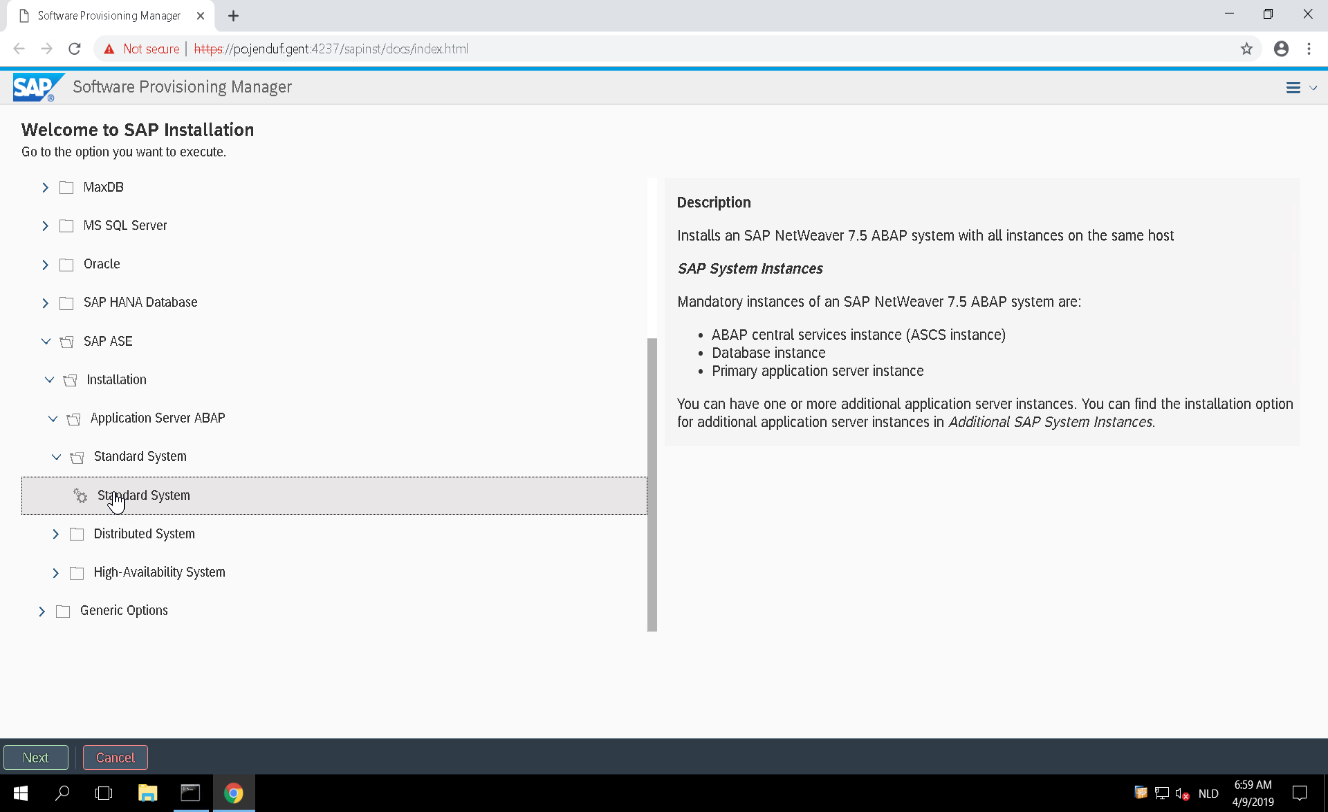
\includegraphics[width=0.9\linewidth]{img/Methodologie/SAP35.png} 
        \centering
        \caption{Select the Standard System}
    \end{subfigure}
\end{figure}
\begin{figure}[!htb]\ContinuedFloat
    \begin{subfigure}{0.5\textwidth}
        \captionsetup{width=0.8\linewidth}
        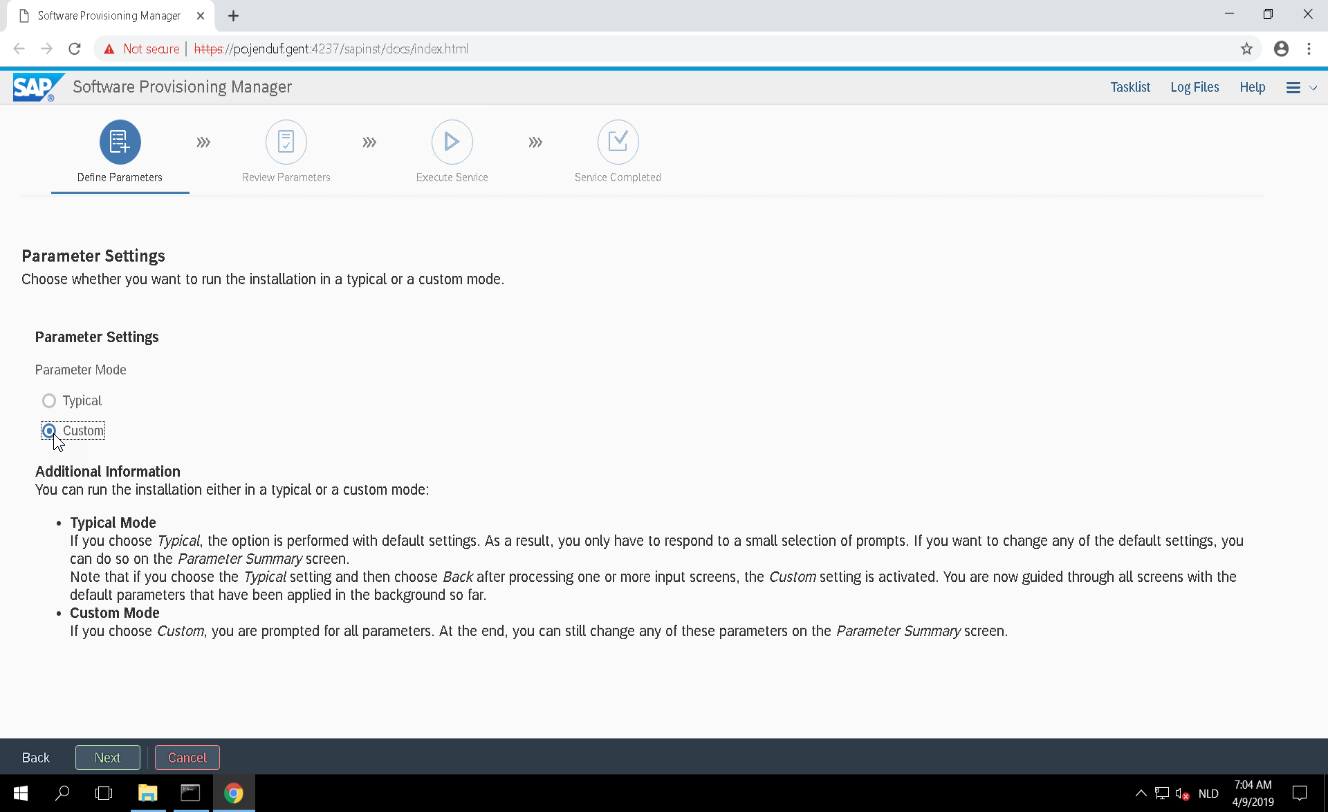
\includegraphics[width=0.9\linewidth]{img/Methodologie/SAP34.png}
        \centering
        \caption{Select the Custom Parameter Settings}
    \end{subfigure}
    \begin{subfigure}{0.5\textwidth}
        \captionsetup{width=0.8\linewidth}
        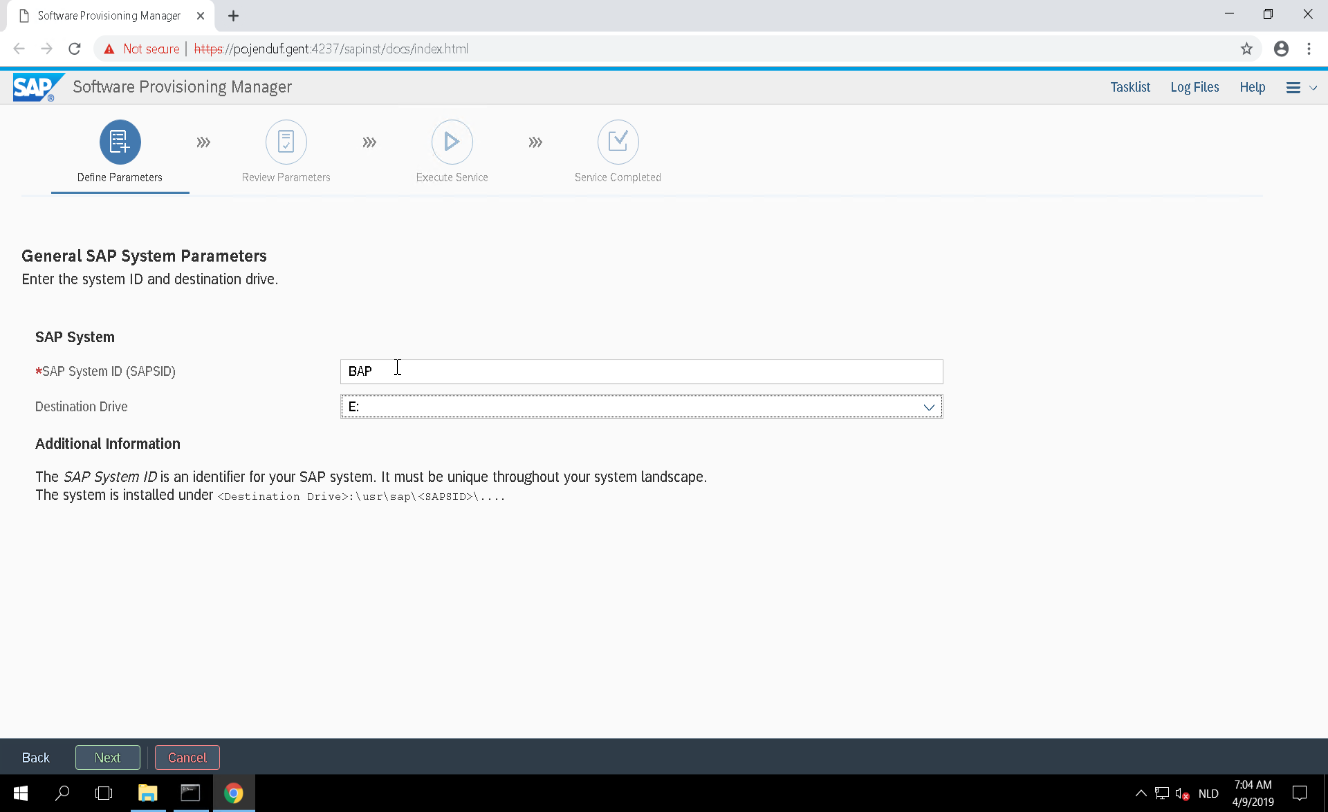
\includegraphics[width=0.9\linewidth]{img/Methodologie/SAP33.png} 
        \centering
        \caption{Enter a SAP System ID and select the Destination Drive}
    \end{subfigure}
\end{figure}
\begin{figure}[!htb]\ContinuedFloat
    \begin{subfigure}{0.5\textwidth}
        \captionsetup{width=0.8\linewidth}
        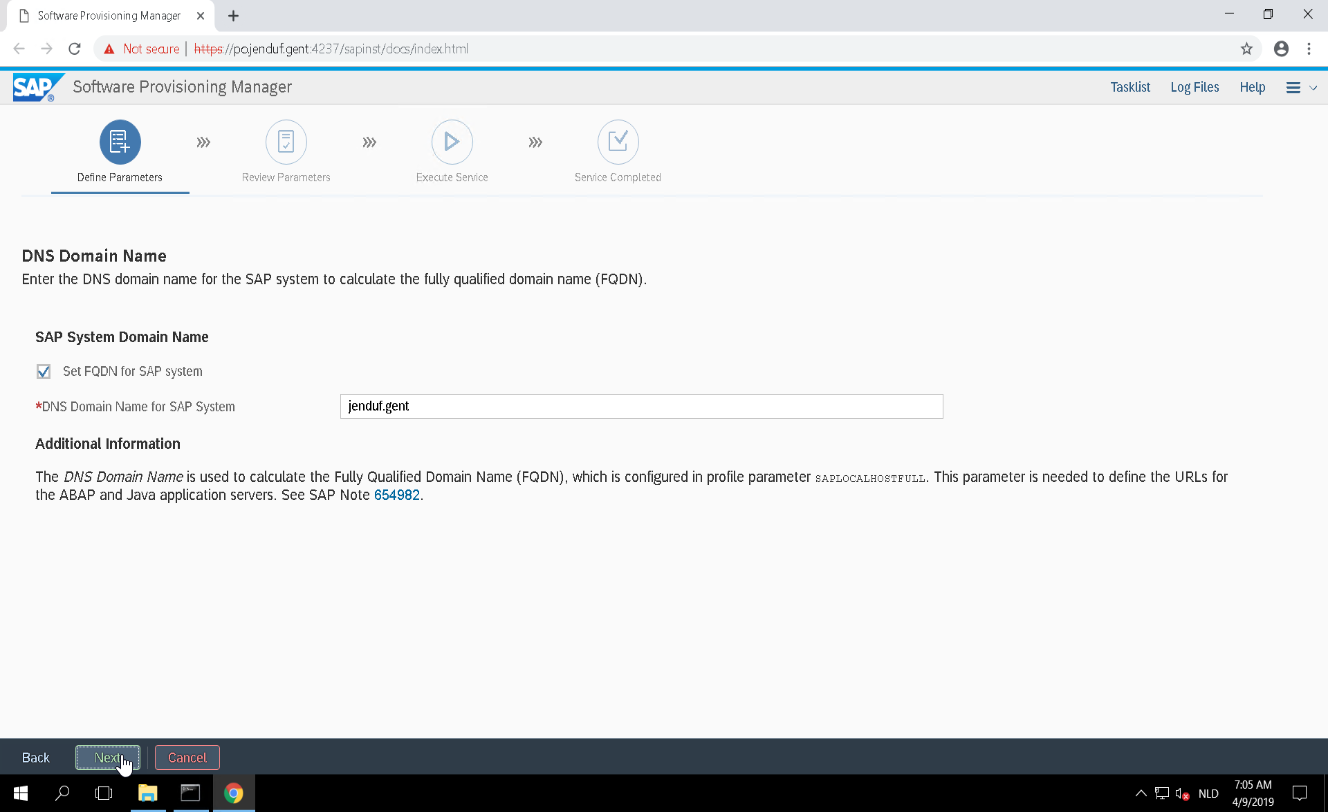
\includegraphics[width=0.9\linewidth]{img/Methodologie/SAP32.png}
        \centering
        \caption{Verify the DNS Domain Name}
    \end{subfigure}
    \begin{subfigure}{0.5\textwidth}
        \captionsetup{width=0.8\linewidth}
        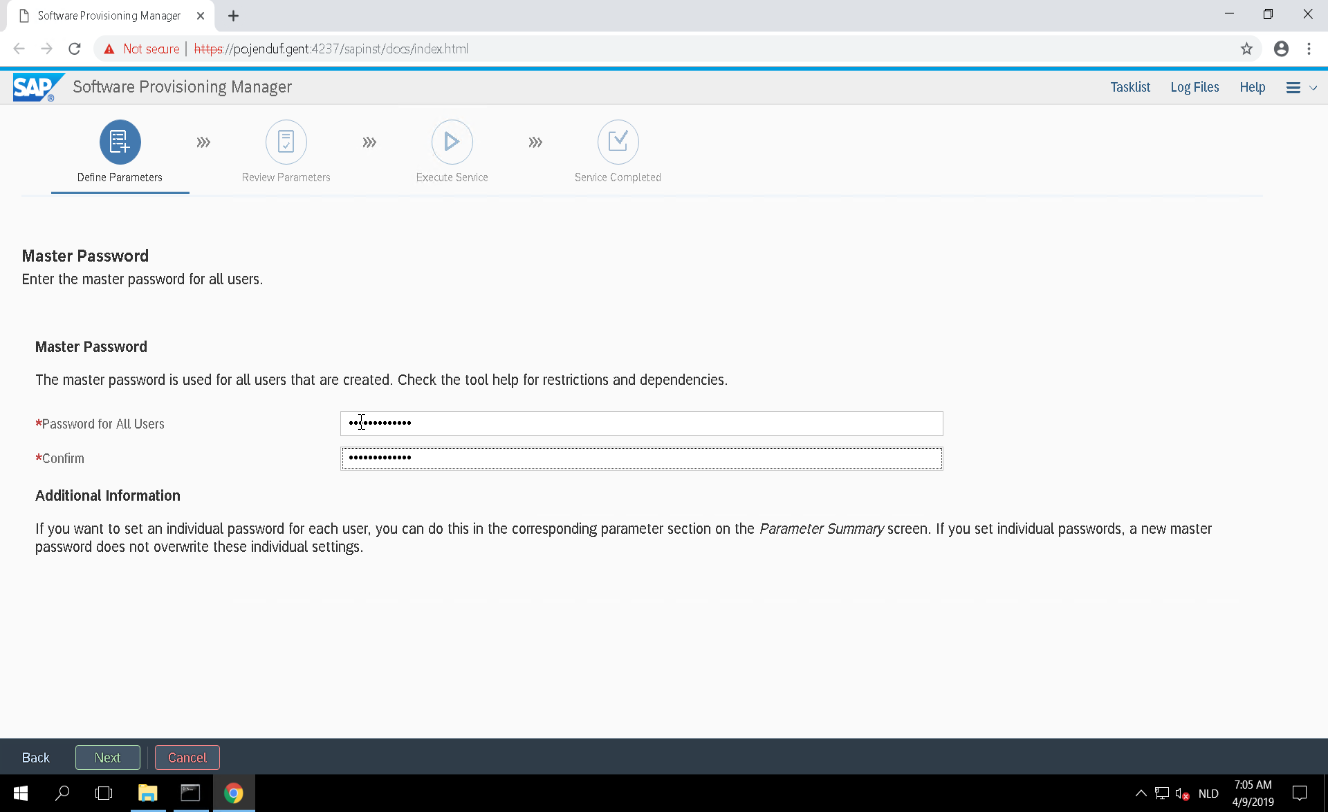
\includegraphics[width=0.9\linewidth]{img/Methodologie/SAP31.png} 
        \centering
        \caption{Enter a Master Password}
    \end{subfigure}
\end{figure}
\begin{figure}[!htb]\ContinuedFloat
    \begin{subfigure}{0.5\textwidth}
        \captionsetup{width=0.8\linewidth}
        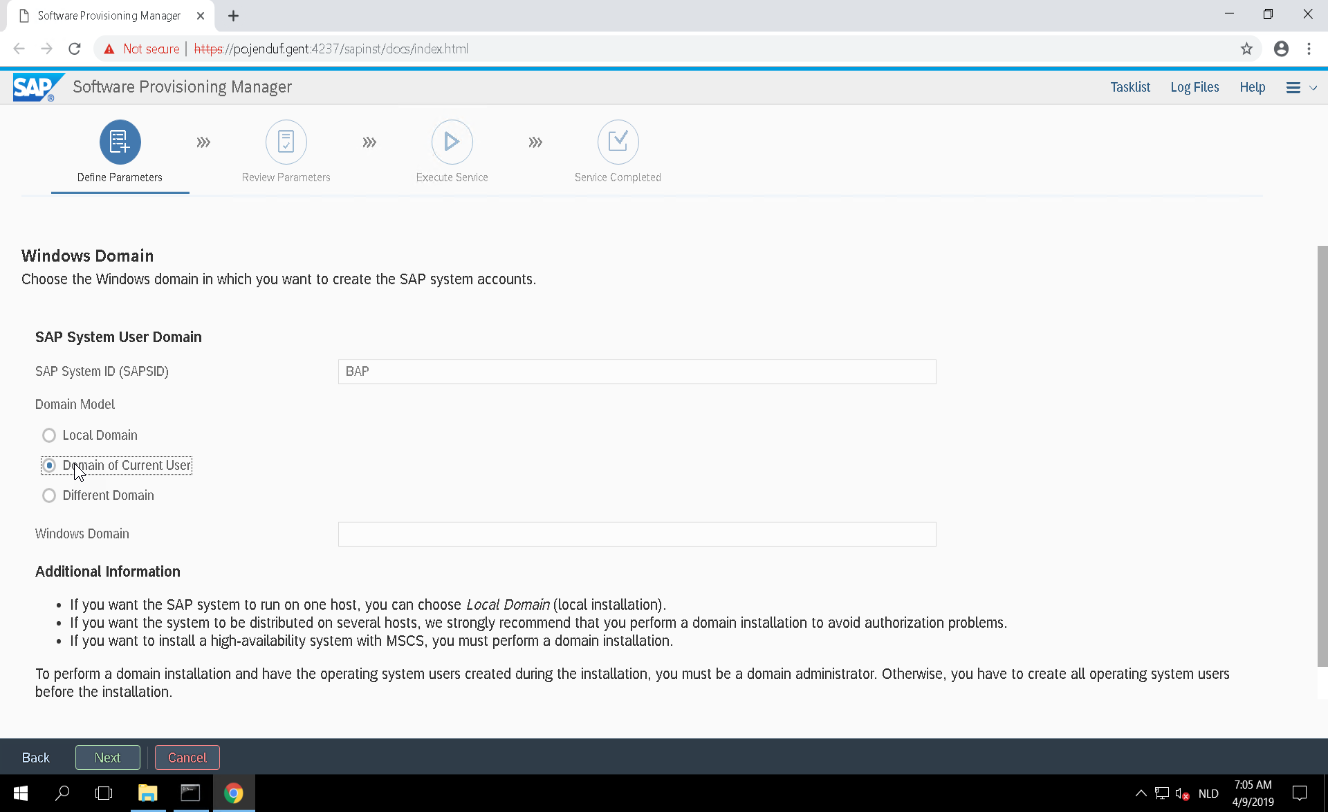
\includegraphics[width=0.9\linewidth]{img/Methodologie/SAP30.png}
        \centering
        \caption{Create the SAP system accounts to the domain of the current user}
    \end{subfigure}
    \begin{subfigure}{0.5\textwidth}
        \captionsetup{width=0.8\linewidth}
        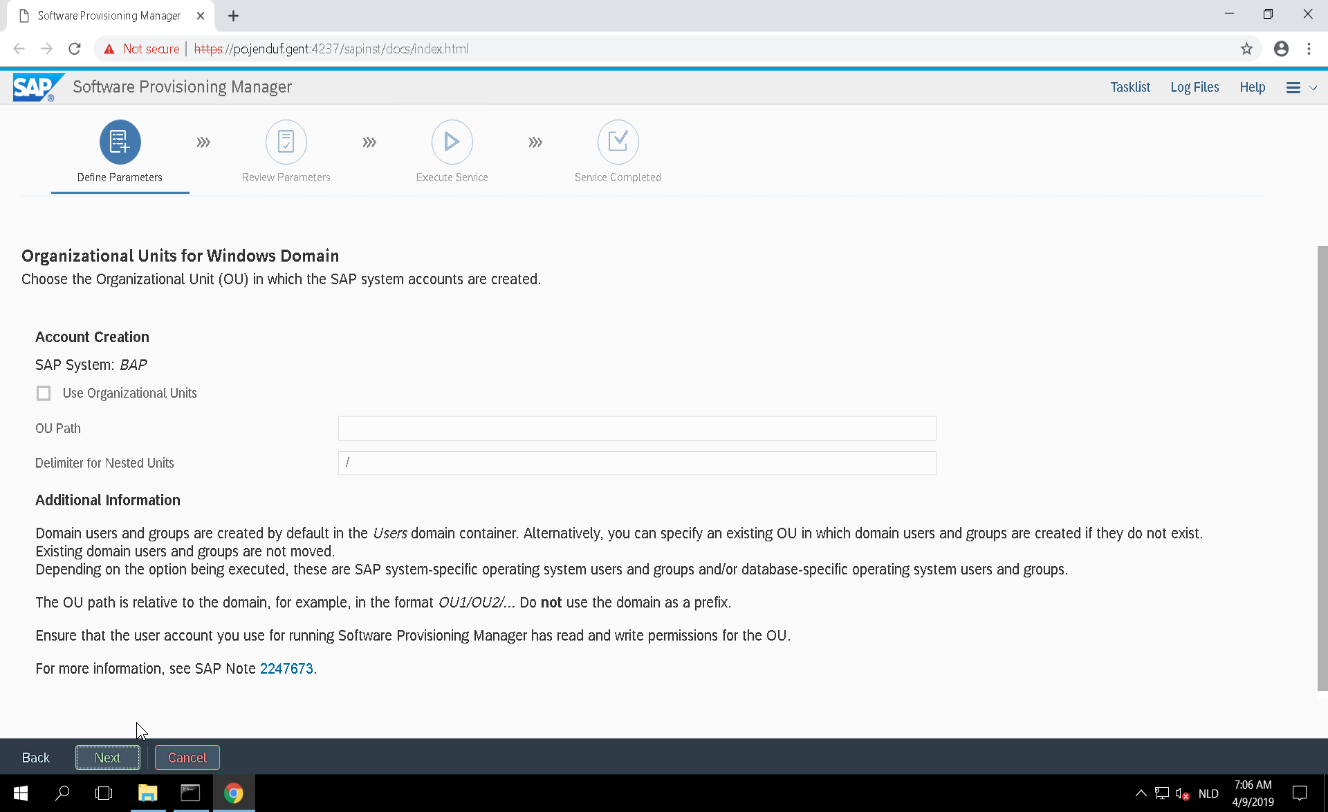
\includegraphics[width=0.9\linewidth]{img/Methodologie/SAP29.png} 
        \centering
        \caption{Verify that no Organizational Units are used}
    \end{subfigure}
\end{figure}
\begin{figure}[!htb]\ContinuedFloat
    \begin{subfigure}{0.5\textwidth}
        \captionsetup{width=0.8\linewidth}
        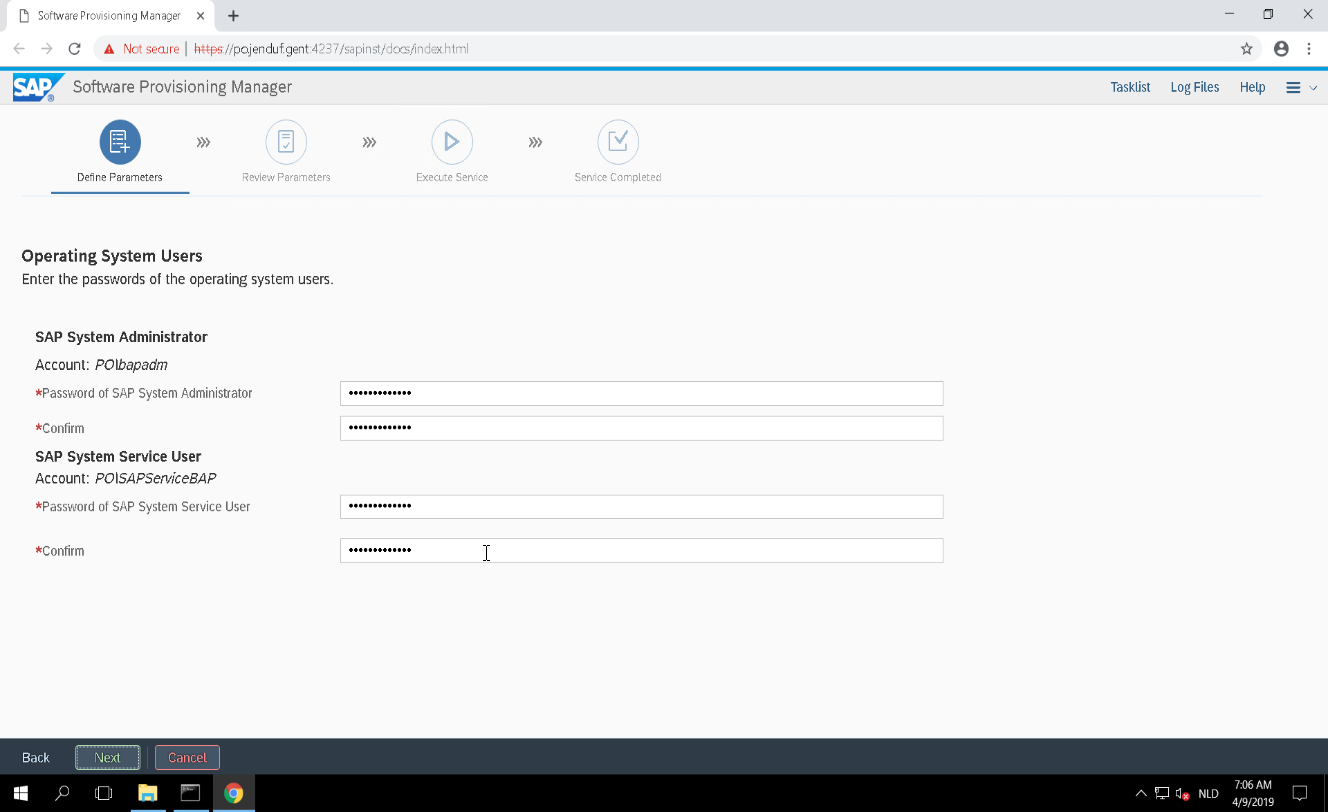
\includegraphics[width=0.9\linewidth]{img/Methodologie/SAP28.png}
        \centering
        \caption{Enter the System Administrator and Service User password}
    \end{subfigure}
    \begin{subfigure}{0.5\textwidth}
        \captionsetup{width=0.8\linewidth}
        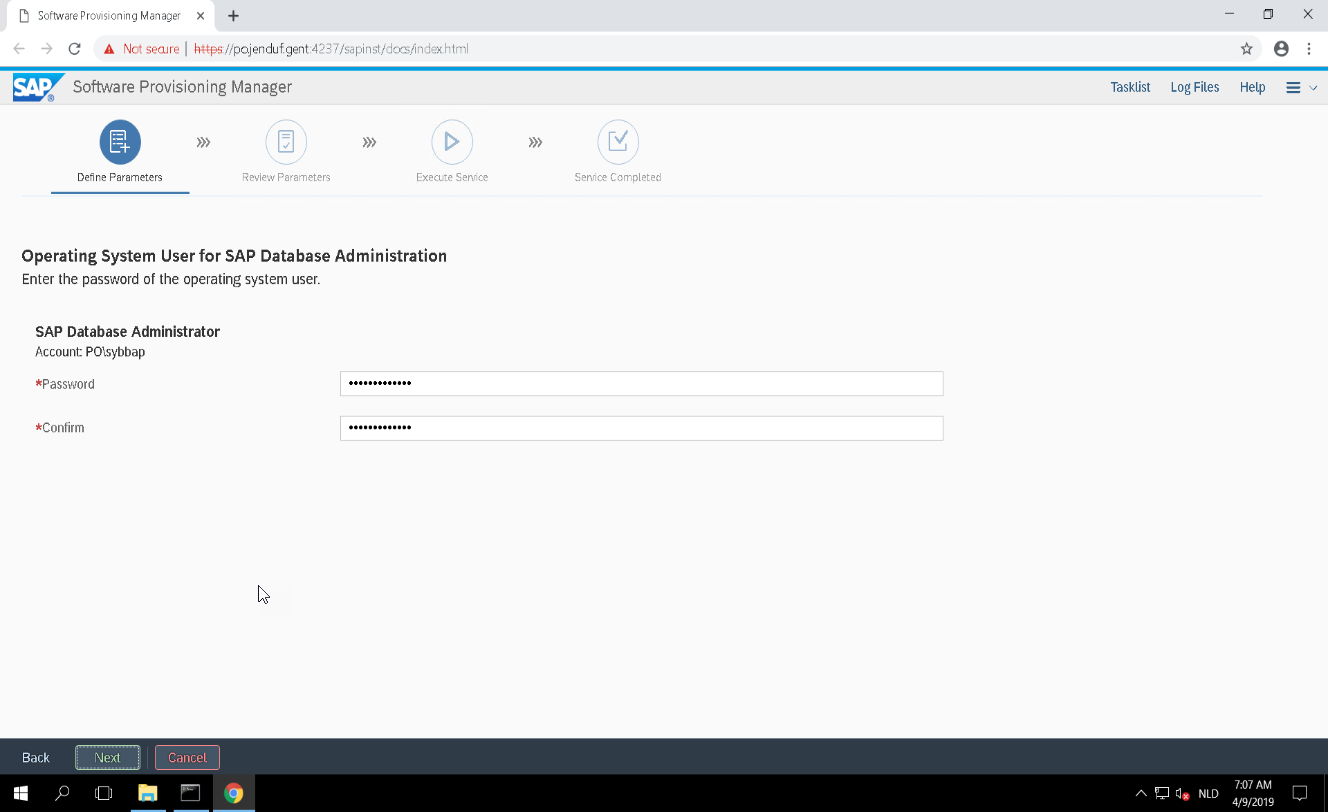
\includegraphics[width=0.9\linewidth]{img/Methodologie/SAP27.png} 
        \centering
        \caption{Enter the SAP Database Administrator password}
    \end{subfigure}
\end{figure}
\begin{figure}[!htb]\ContinuedFloat
    \begin{subfigure}{0.5\textwidth}
        \captionsetup{width=0.8\linewidth}
        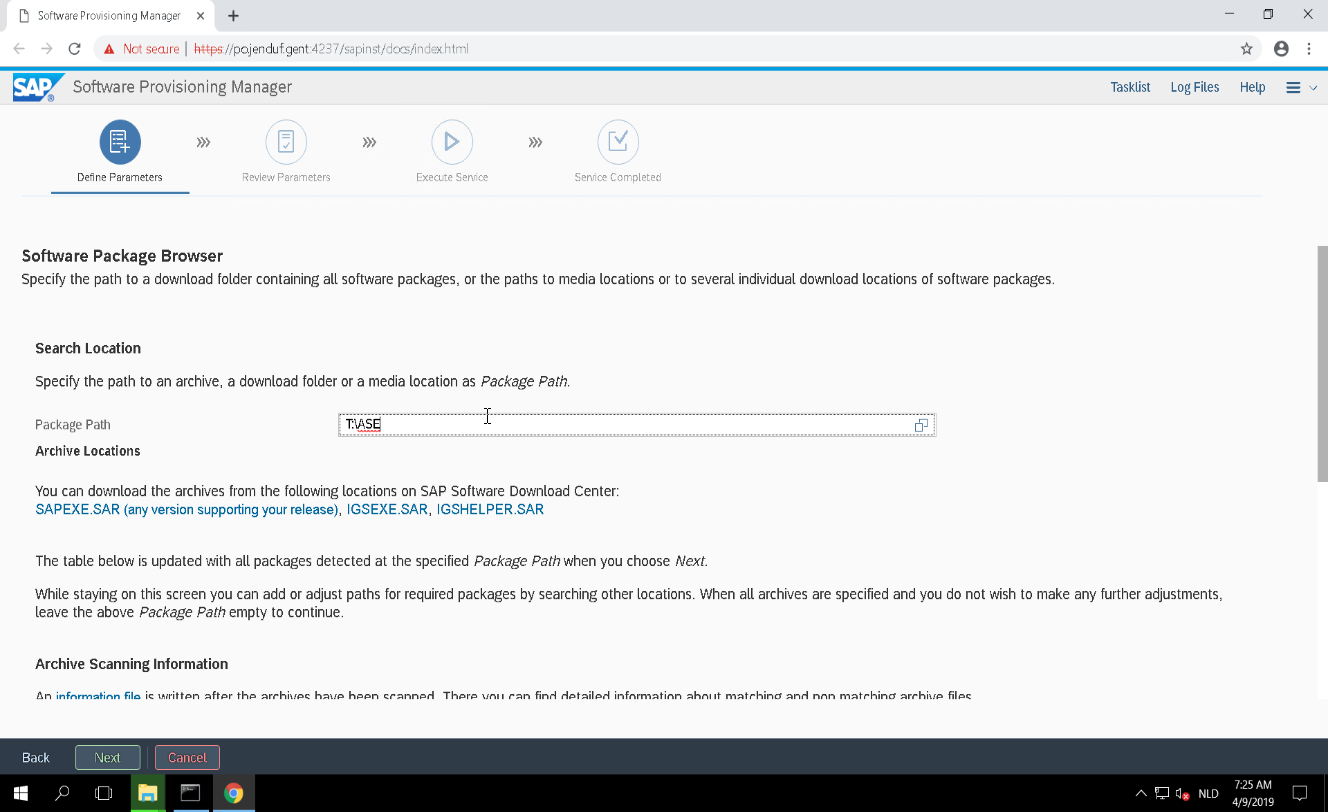
\includegraphics[width=0.9\linewidth]{img/Methodologie/SAP26.png}
        \centering
        \caption{Enter the Package Path}
    \end{subfigure}
    \begin{subfigure}{0.5\textwidth}
        \captionsetup{width=0.8\linewidth}
        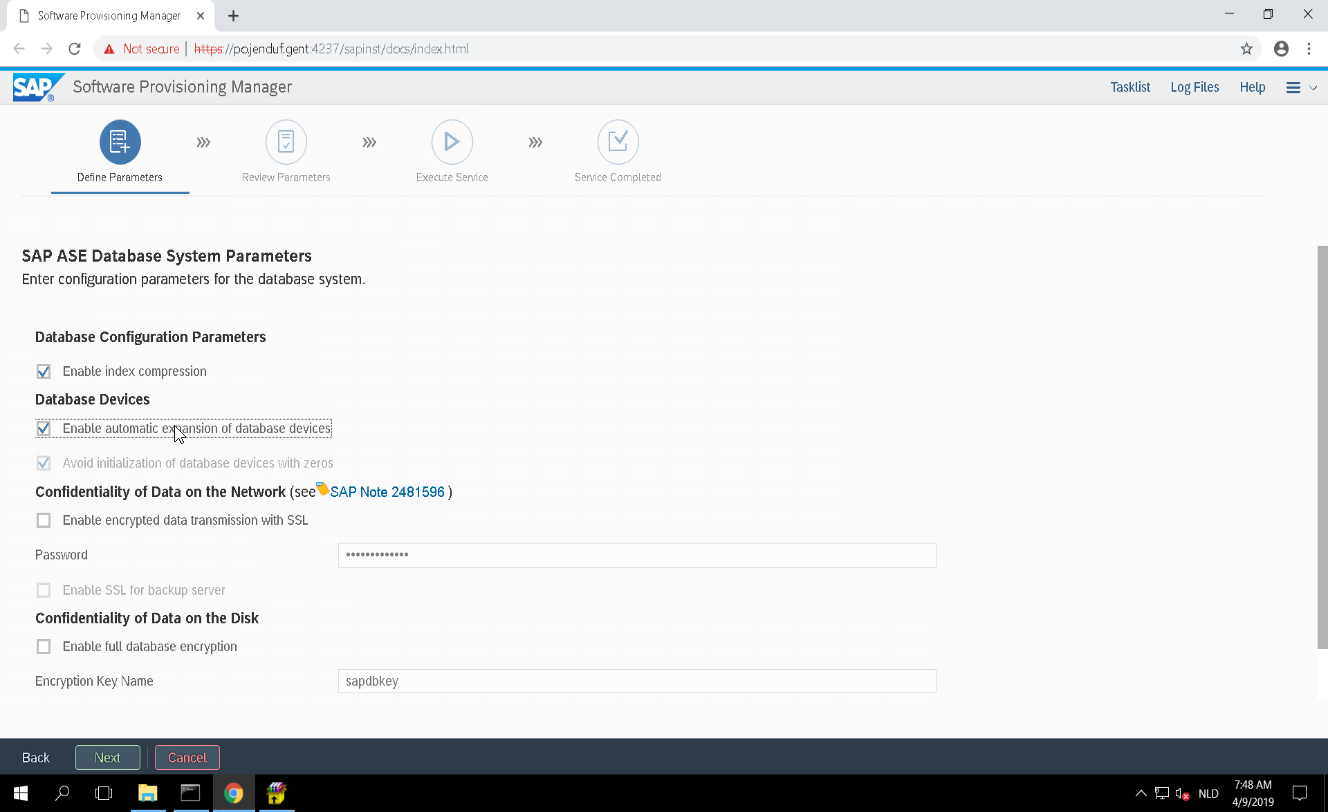
\includegraphics[width=0.9\linewidth]{img/Methodologie/SAP22.png}
        \centering
        \caption{Enable automatic expansion of database devices}
\end{subfigure}
\end{figure}
\begin{figure}[!htb]\ContinuedFloat
    \begin{subfigure}{0.5\textwidth}
        \captionsetup{width=0.8\linewidth}
        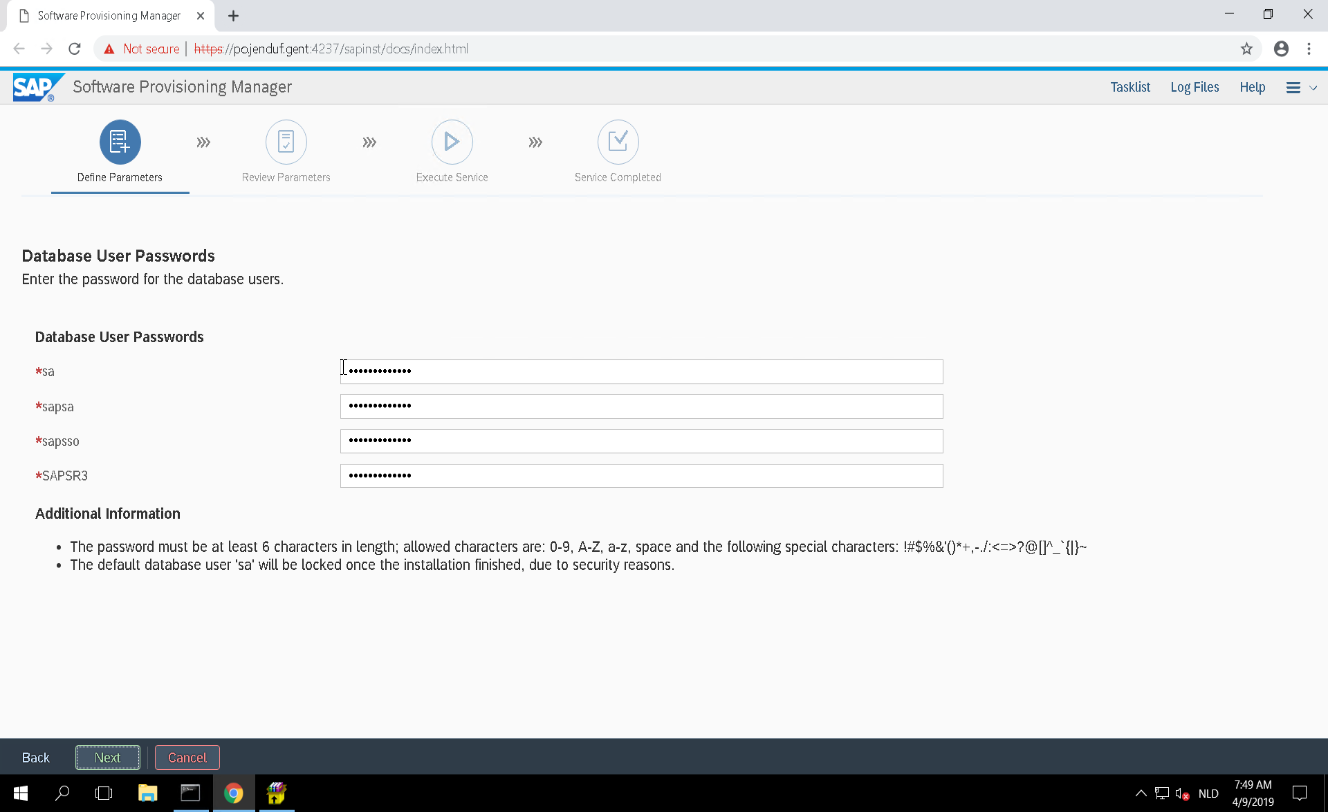
\includegraphics[width=0.9\linewidth]{img/Methodologie/SAP18.png}
        \centering
        \caption{Enter the Database User Passwords}
    \end{subfigure}
    \begin{subfigure}{0.5\textwidth}
    \captionsetup{width=0.8\linewidth}
    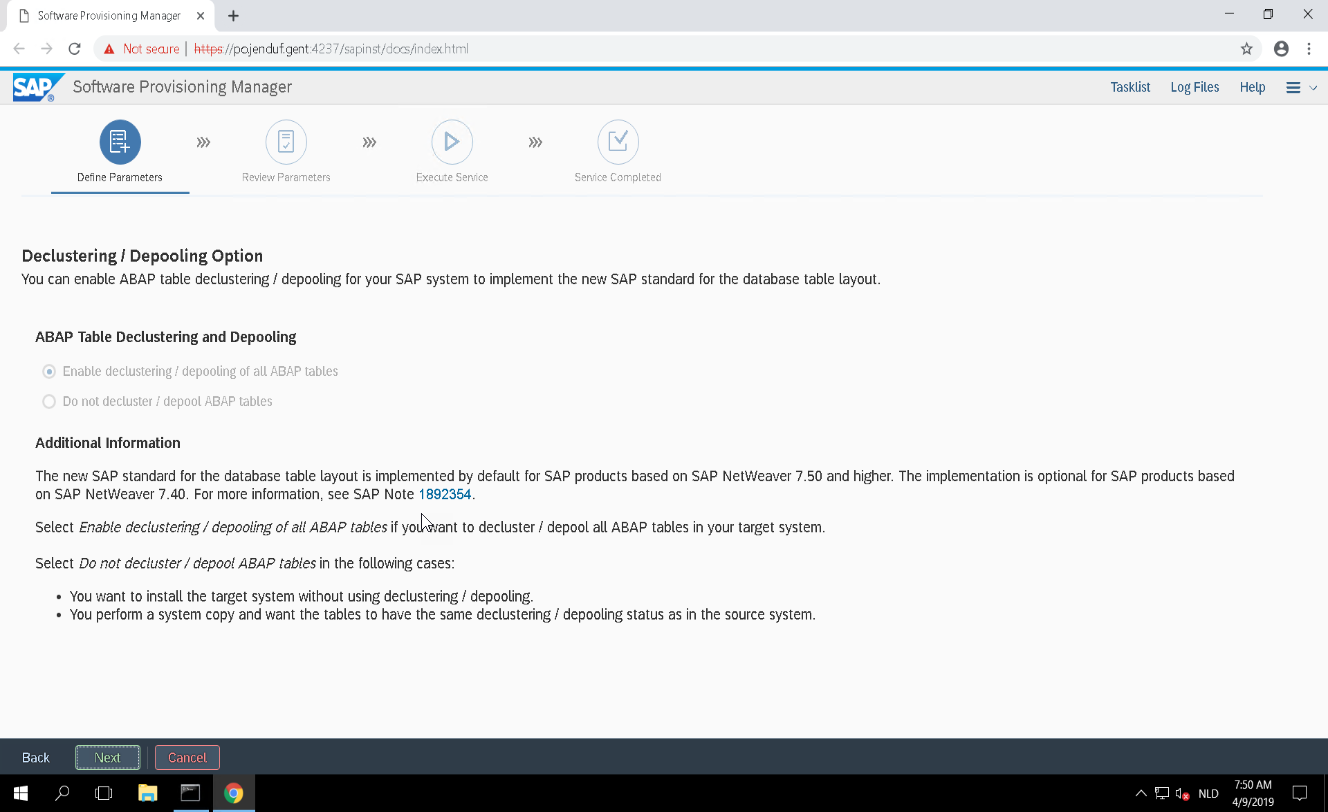
\includegraphics[width=0.9\linewidth]{img/Methodologie/SAP16.png}
    \centering
    \caption{Click next}
    \end{subfigure}
\end{figure}
\begin{figure}[!htb]\ContinuedFloat
    \begin{subfigure}{0.5\textwidth}
        \captionsetup{width=0.8\linewidth}
        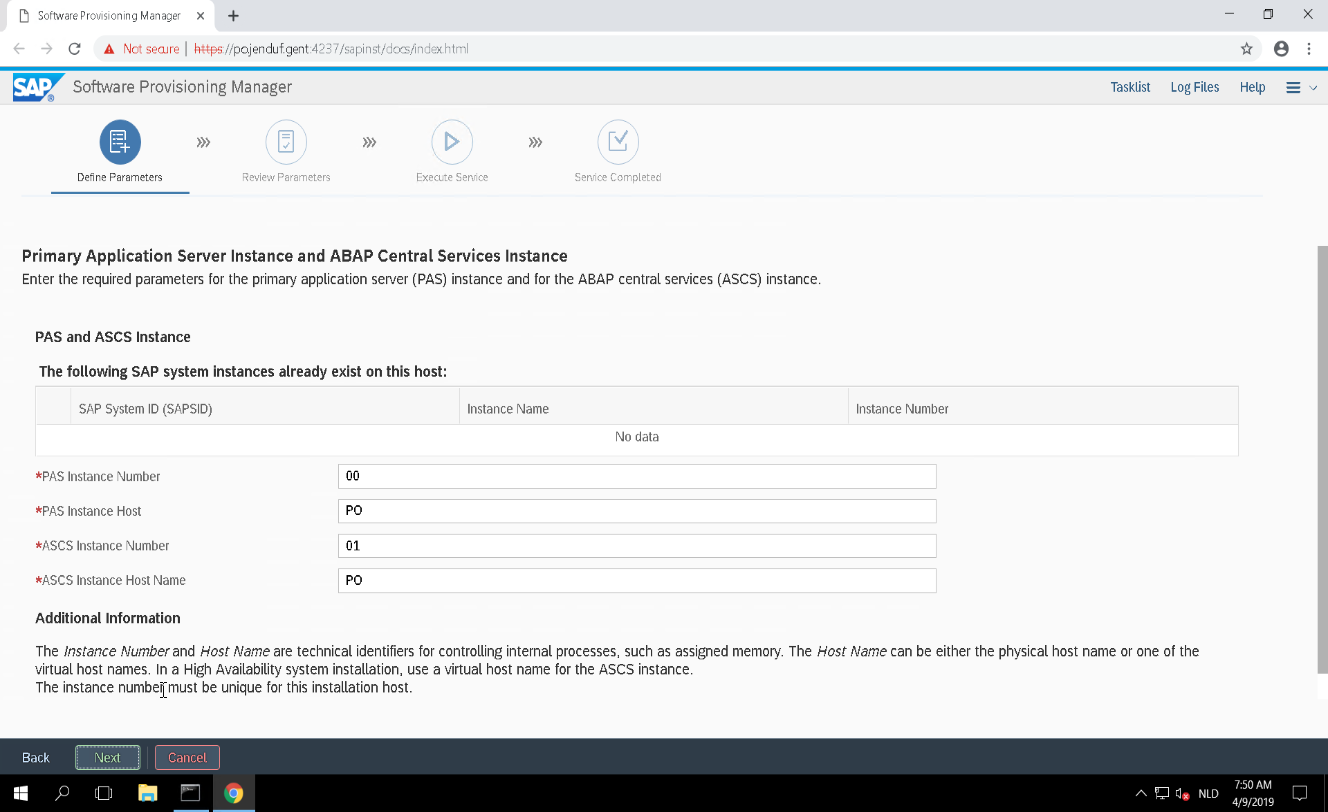
\includegraphics[width=0.9\linewidth]{img/Methodologie/SAP14.png}
        \centering
        \caption{Verify that no SAP system instances already exist}
    \end{subfigure}
    \begin{subfigure}{0.5\textwidth}
    \captionsetup{width=0.8\linewidth}
    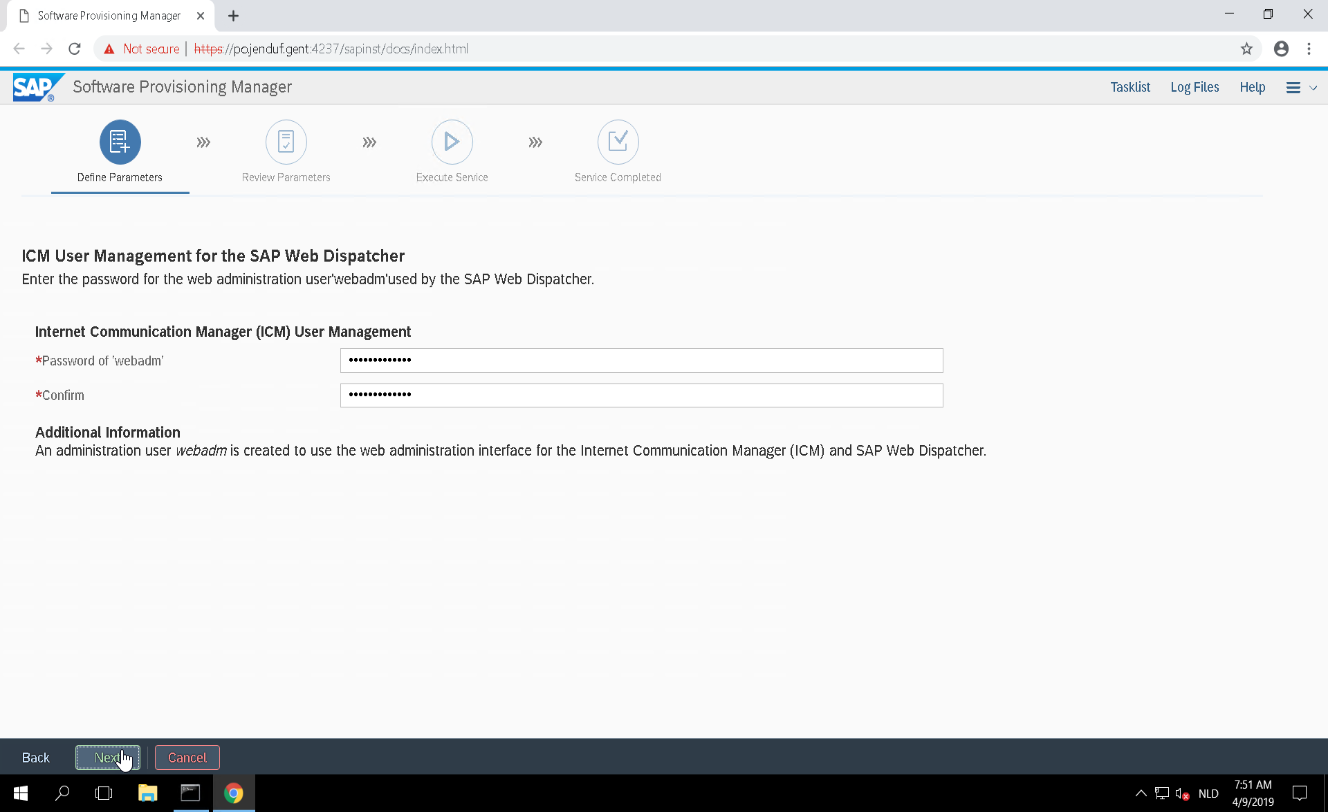
\includegraphics[width=0.9\linewidth]{img/Methodologie/SAP12.png}
    \centering
    \caption{Enter the webadmin password}
    \end{subfigure}
\end{figure}
\begin{figure}[!htb]\ContinuedFloat
    \begin{subfigure}{0.5\textwidth}
        \captionsetup{width=0.8\linewidth}
        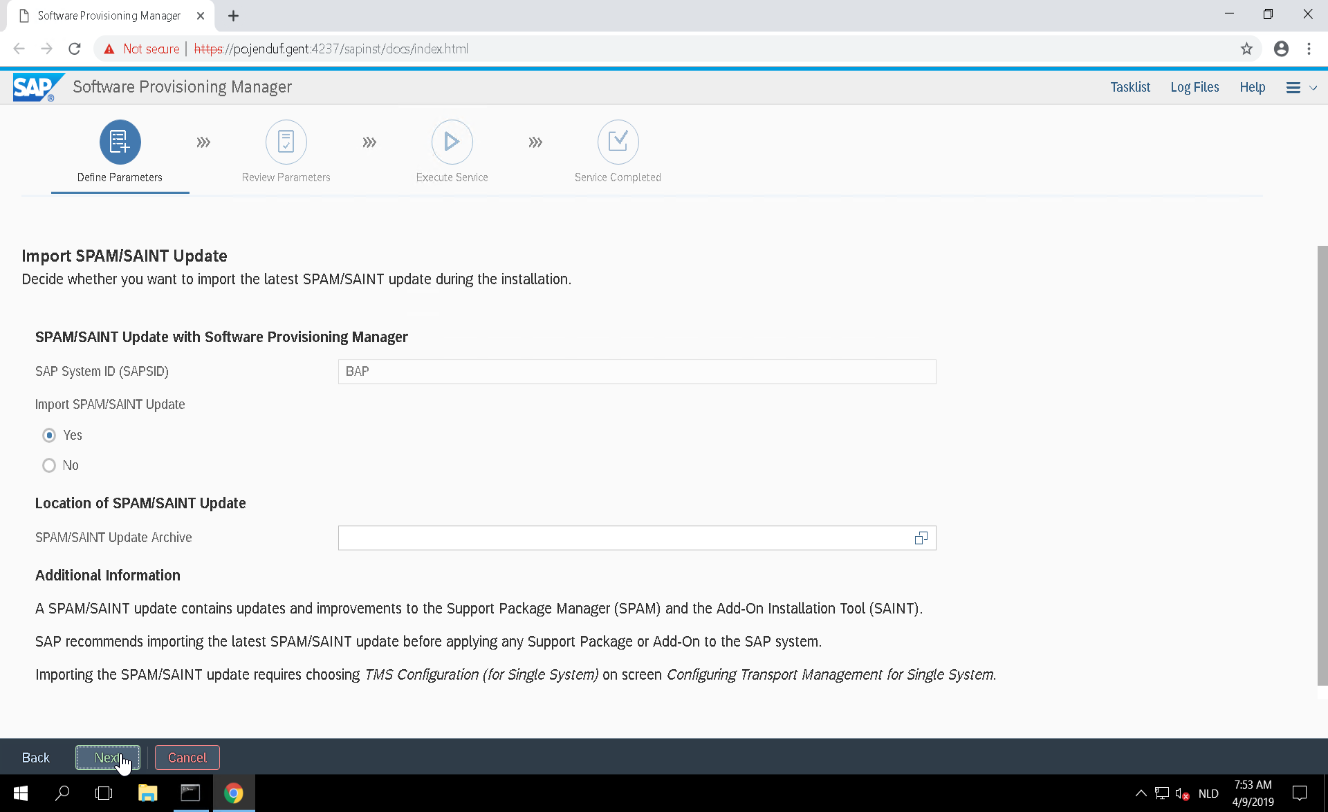
\includegraphics[width=0.9\linewidth]{img/Methodologie/SAP07.png} 
        \centering
        \caption{Disable Import SPAM/SAINT Update}
    \end{subfigure}
    \begin{subfigure}{0.5\textwidth}
    \captionsetup{width=0.8\linewidth}
    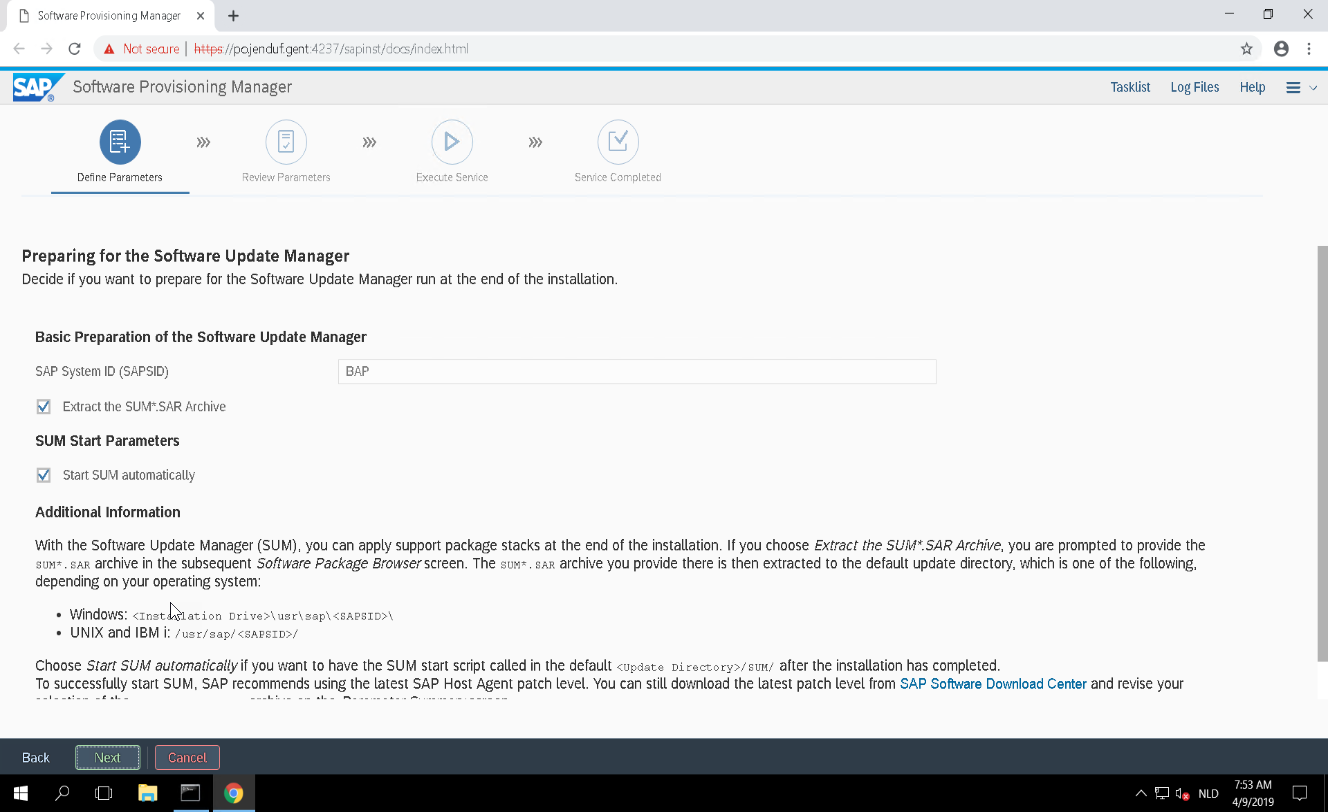
\includegraphics[width=0.9\linewidth]{img/Methodologie/SAP05.png} 
    \centering
    \caption{Verify the Software Update Manager configuration}
\end{subfigure}
\end{figure}
\begin{figure}[!htb]\ContinuedFloat
    \begin{subfigure}{0.5\textwidth}
        \captionsetup{width=0.8\linewidth}
        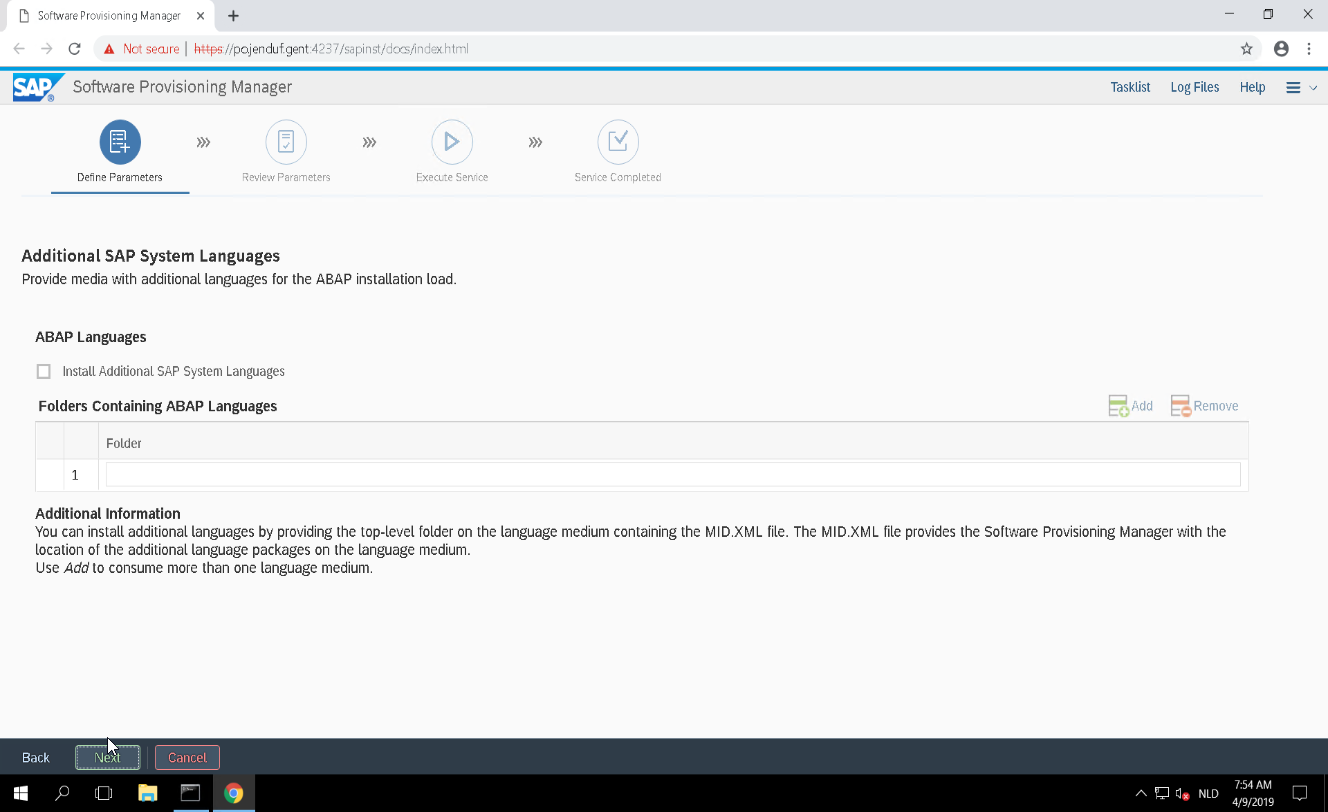
\includegraphics[width=0.9\linewidth]{img/Methodologie/SAP04.png}
        \centering
        \caption{Verify the installation of additional SAP System Languages}
    \end{subfigure}
    \begin{subfigure}{0.5\textwidth}
        \captionsetup{width=0.8\linewidth}
        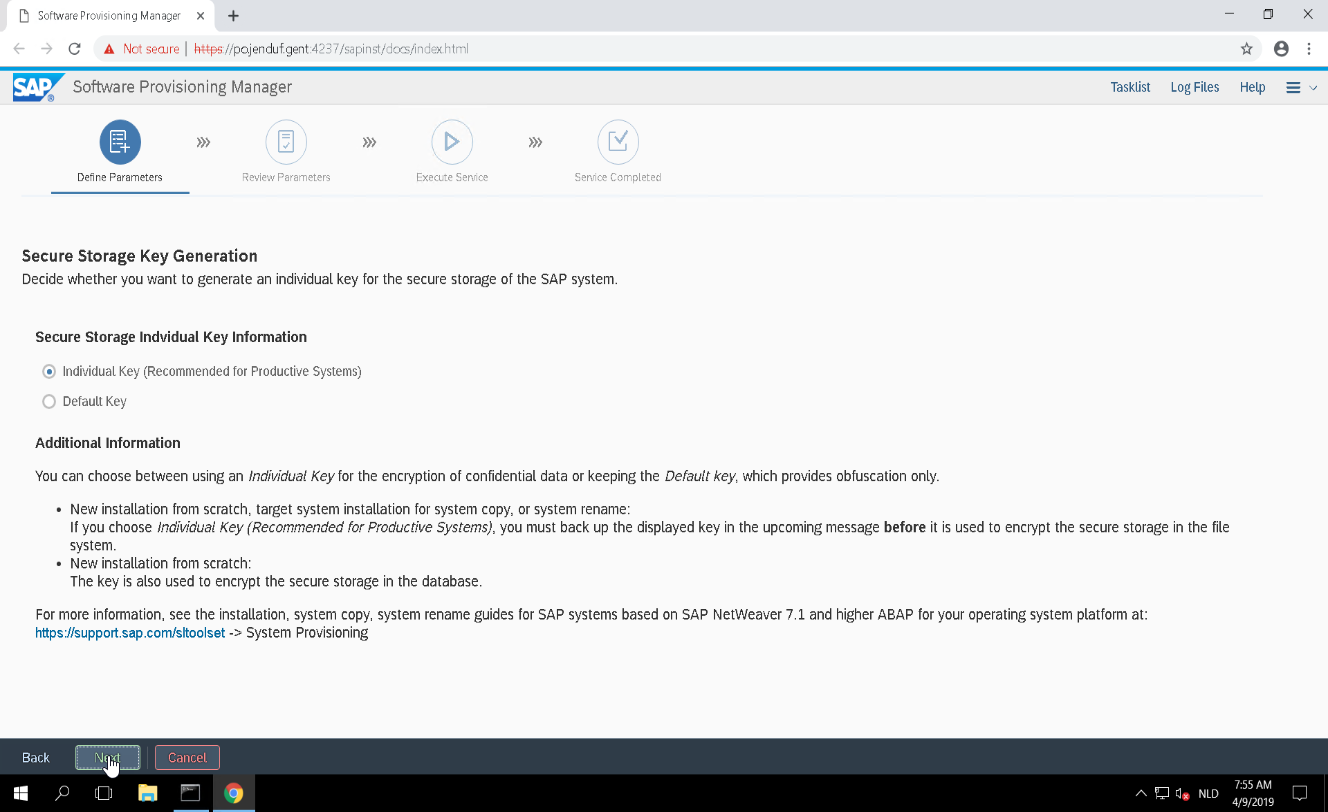
\includegraphics[width=0.9\linewidth]{img/Methodologie/SAP03.png} 
        \centering
        \caption{Generate the Secure Storage Key}
    \end{subfigure}
\end{figure}
\begin{figure}[!htb]\ContinuedFloat
    \begin{subfigure}{0.5\textwidth}
        \captionsetup{width=0.8\linewidth}
        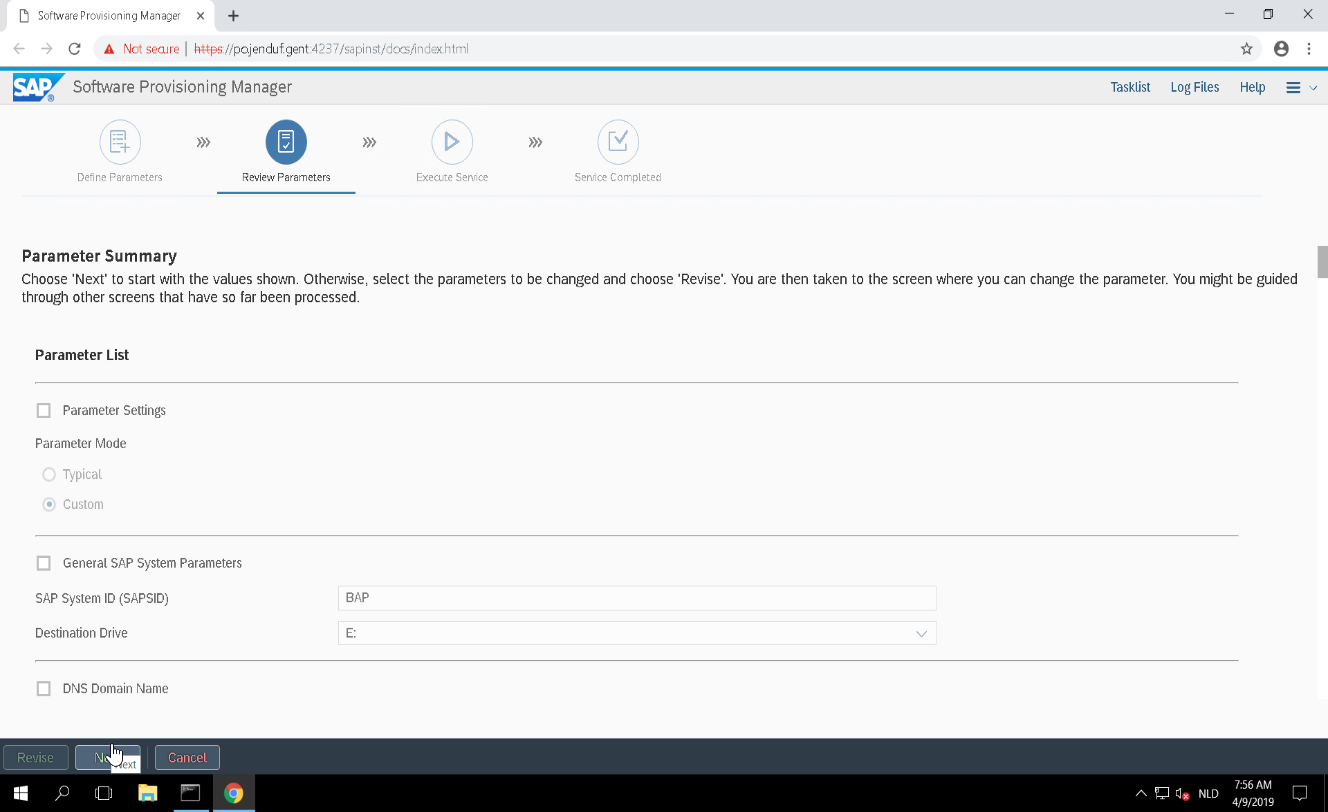
\includegraphics[width=0.9\linewidth]{img/Methodologie/SAP01.png}
        \centering
        \caption{Review all the Parameters in the summary}
    \end{subfigure}
    \begin{subfigure}{0.5\textwidth}
        \captionsetup{width=0.8\linewidth}
        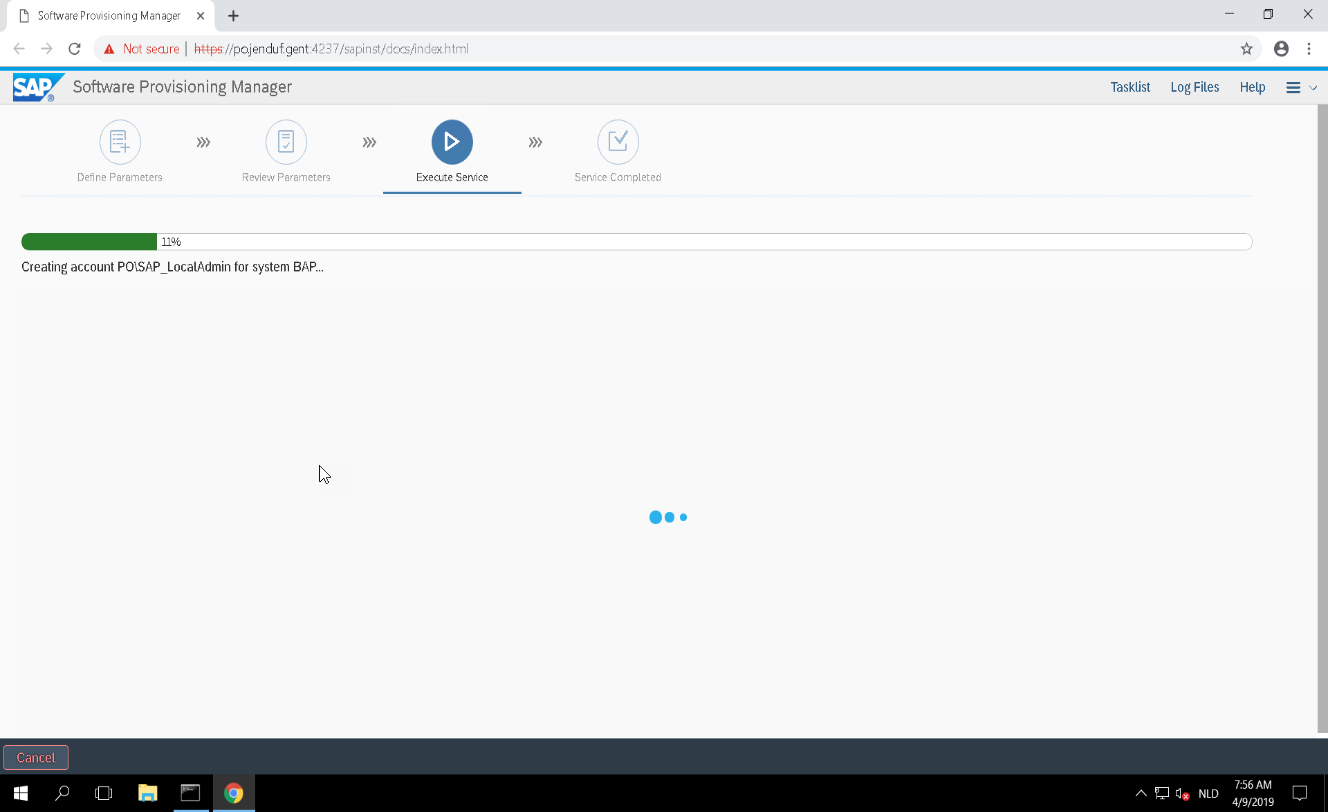
\includegraphics[width=0.9\linewidth]{img/Methodologie/SAP00.png} 
        \centering
        \caption{The installation has successfully started}
    \end{subfigure}
    \caption[Installation SAP]{Installation of the SAP application server with SyBase ASE DB}
\end{figure}